\section{Introduction}
After completing the design phase of the application, we will begin in this chapter the realization and implementation part by explaining the work environment and the selected development tools as well as the interfaces of our application.

At the end of this chapter, the objectives must have been achieved and the system must be ready to be exploited by end users.




\section{Development environment}

For the realization of our application, we used different tools and development software, tool for database management, modeling software, software for writing this report


\subsection{Adobe XD}
Adobe XD is a user experience design tool used to create wireframes, prototypes, and designs for digital products. It includes design and prototyping tools, collaboration features, and the ability to design for multiple devices and screen sizes. It's part of Adobe Creative Cloud, a subscription-based service for creative tools and services. \cite{adobe}
\begin{figure}[H]
    \centering
    
\includegraphics[width=0.3\textwidth]{images/Adobe_XD_CC_icon.svg.png}
    \caption{Adobe XD logo}
    \label{fig:figure4}
\end{figure}


\subsection{Visual Studio Code}
Visual Studio Code, also commonly referred to as VS Code, is a source-code editor made by Microsoft with the Electron Framework, for Windows, Linux and macOS.Features include support for debugging, syntax highlighting, intelligent code completion, snippets, code refactoring, and embedded Git. Users can change the theme, keyboard shortcuts, preferences, and install extensions that add functionality.

In the Stack Overflow 2022 Developer Survey, Visual Studio Code was ranked the most popular developer environment tool among 71,010 respondents, with 74.48 reporting that they use it.\cite{vscode}

\begin{figure}[H]
    \centering
    
\includegraphics[width=0.6\textwidth]{images/1_EOPCay4ML76rIUskd6ZwRg.png}
    \caption{visual studio code logo}
    \label{fig:figure4}
\end{figure}

\subsection{Flutter Framwork}
Flutter is an open-source mobile application development framework created by Google that allows developers to build native-looking, high-performance mobile applications for Android, iOS, and other platforms, using a single codebase. It's known for its ease of use, fast development times, and ability to create beautiful and responsive UI designs. \cite{flutter}
\begin{figure}[H]
    \centering
    
\includegraphics[width=0.5\textwidth]{images/c823e53b3a1a7b0d36a9.png}
    \caption{flutter logo}
    \label{fig:figure4}
\end{figure}

\subsection{Dart Language}
Dart is a general-purpose, object-oriented programming language created by Google that's designed to be fast, efficient, and easy to learn. It's used for a wide range of applications, from web and mobile development to server-side programming, and is the primary language used to develop applications with Google's Flutter framework.\cite{dart}
\begin{figure}[H]
    \centering
    
\includegraphics[width=0.5\textwidth]{images/Dart_programming_language_logo.svg.png}
    \caption{dart language logo}
    \label{fig:figure4}
\end{figure}

\subsection{Firebase}
Firebase is a cloud-based mobile and web application development platform developed by Google that provides a comprehensive set of services and tools to help developers build high-quality, scalable applications quickly and easily. It includes a real-time database, authentication, hosting, cloud functions, and more, and enables developers to store and manage data in real-time, run server-side code in response to events, and deploy web applications to the cloud with ease.\cite{firebase}
\begin{figure}[H]
    \centering
    
\includegraphics[width=0.5\textwidth]{images/512px-Firebase_Logo.svg.png}
    \caption{firebase logo}
    \label{fig:figure4}
\end{figure}

\subsection{BlueStacks}
BlueStacks is a popular Android emulator software that allows users to run Android applications on their desktop or laptop computers. It creates a virtual Android device on the user's computer, enabling them to interact with Android apps using their mouse, keyboard, and other peripherals. BlueStacks supports a wide range of Android apps and provides a seamless and immersive Android experience on desktop and laptop computers.\cite{bluestacks}
\begin{figure}[h]
    \centering
    
\includegraphics[width=0.5\textwidth]{images/e634679eb4e06627c42ca5667d83e88e.png}
    \caption{BlueStacks logo}
    \label{fig:figure4}
\end{figure}

\subsection{StarUML}
StarUML is a popular open-source UML modeling tool that helps developers create high-quality software designs using a variety of UML diagrams. It provides advanced features such as model validation, code generation, and round-trip engineering, and is widely used in software development projects for its flexibility, extensibility, and ease-of-use. StarUML is available for Windows, Mac, and Linux platforms and helps developers create high-quality software designs efficiently and effectively.
\begin{figure}[h]
    \centering
    
\includegraphics[width=0.5\textwidth]{images/Ey8OGaPWUAAfrVX.jpg}
    \caption{StarUML logo}
    \label{fig:figure4}
\end{figure}


\subsection{Latex }
The report was written using LaTeX, which is both a language and a document composition system. It allows for automatic document layout adhering to typographical norms, and is known for its mathematical mode which allows for complex formulas to be easily composed. LaTeX is popular in technical and scientific fields, and is often used for medium or large-sized documents such as articles, theses, and books.
\begin{figure}[H]
    \centering
    
\includegraphics[width=0.5\textwidth]{images/latex-logo-png-transparent.png}
    \caption{Latex logo}
    \label{fig:figure4}
\end{figure}

\subsection{Overleaf }

Overleaf is a web-based platform for writing and collaborating on LaTeX documents. It offers a variety of features including real-time collaboration, automatic document backups, and a wide range of templates and examples. Overleaf simplifies the process of writing LaTeX documents by providing an intuitive user interface and a variety of helpful tools and resources. In our case, we used Overleaf to write and collaborate on this report, taking advantage of its features and functionality to streamline the writing and editing document and save it PDF.\cite{overleaf}
\begin{figure}[H]
    \centering
    
\includegraphics[width=0.5\textwidth]{images/overleaf_wide_colour_light_bg.png}
    \caption{Latex logo}
    \label{fig:figure4}
\end{figure}



\section{Graphic Charter}
The graphic chart and design of an app play a crucial role in creating a strong visual identity and enhancing user experience,conveying the app's message, and enhancing usability for donors and users,in this part we will see what we used in our application "drop angel" .
    \begin{figure}[H]
    \centering
    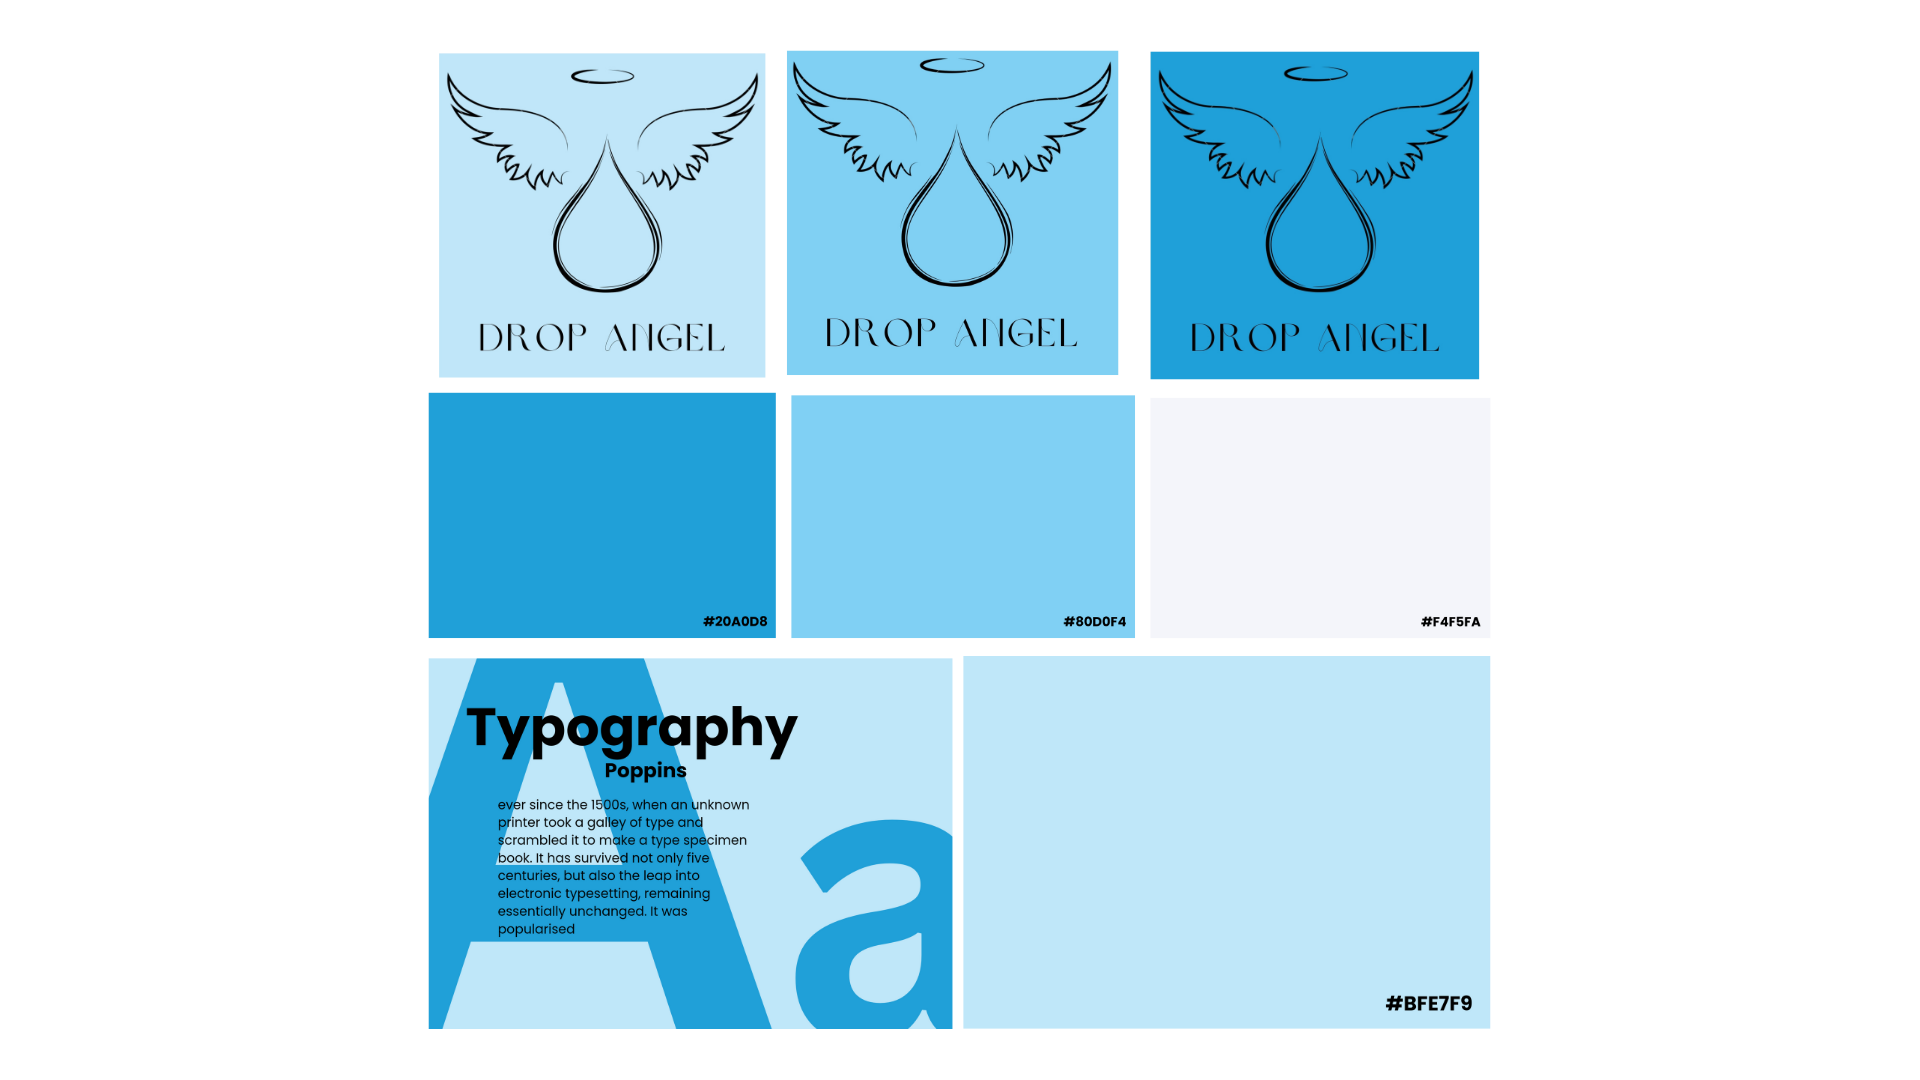
\includegraphics[width=1.15\textwidth]{images/Let's brainstorm for thoughts, ideas, and inspiration using an idea board. (3).png}
    \caption{graphic charter}
    \label{fig:figure4}
\end{figure}


\subsection{Colors }
Choosing a specific color scheme for an application can have a significant impact on user engagement and overall brand identity. In the case of a blood donation app, the color blue can be a compelling choice. Blue is often associated with trust, reliability, and professionalism, making it an ideal color for a healthcare-related application. Additionally, blue is known to have a calming effect on the mind and body, which can be beneficial for users who may be anxious or hesitant about donating blood. Overall, the choice of blue as the primary color for a blood donation app can help to establish a sense of trust, professionalism, and calmness, while also conveying the seriousness and importance of the cause.


\begin{figure}[H]
\begin{subfigure}{.5\textwidth}
  \centering
  % include first image
  
\includegraphics[width=.9\linewidth]{images/color1.png}  
  \caption{Main color 1}
  \label{fig:sub-first}
\end{subfigure}
\begin{subfigure}{.5\textwidth}
  \centering
  % include second image
  
\includegraphics[width=.9\linewidth]{images/4.png}  
  \caption{Main color 2}
  \label{fig:sub-second}
\end{subfigure}
%\newline %\newline
\begin{subfigure}{.5\textwidth}
  \centering
  % include third image
  
\includegraphics[width=.9\linewidth]{images/3.png} 
  \caption{Main color 3}
  \label{fig:sub-third}
\end{subfigure}
\begin{subfigure}{.5\textwidth}
  \centering
  % include fourth image
  
\includegraphics[width=.9\linewidth]{images/5.png} 
  \caption{Main color 4}
  \label{fig:sub-fourth}
\end{subfigure}
\caption{Main Colors}
\label{fig:fig}
\end{figure}


\subsection{Logo }

\begin{figure}[H]
    \centering
    
\includegraphics[width=0.6\textwidth]{images/logo.png}
    \caption{Drop Angel logo}
    \label{fig:figure4}
\end{figure}
A logo can play a crucial role in creating a strong visual identity and communicating the app's message to its users that why we decided to create a logo for our application "Drop Angel" that features a drop of blood with angel wings,We chose this design because it is a powerful symbol of hope, compassion, and urgency. The combination of the angel wings and the drop of blood can create an emotional connection with users, making them more likely to engage with the app and support its mission. We believe that the logo will effectively convey the message that blood donation can save lives and encourage potential donors to take action.


\subsection{Typography}

\begin{figure}[H]
    \centering
    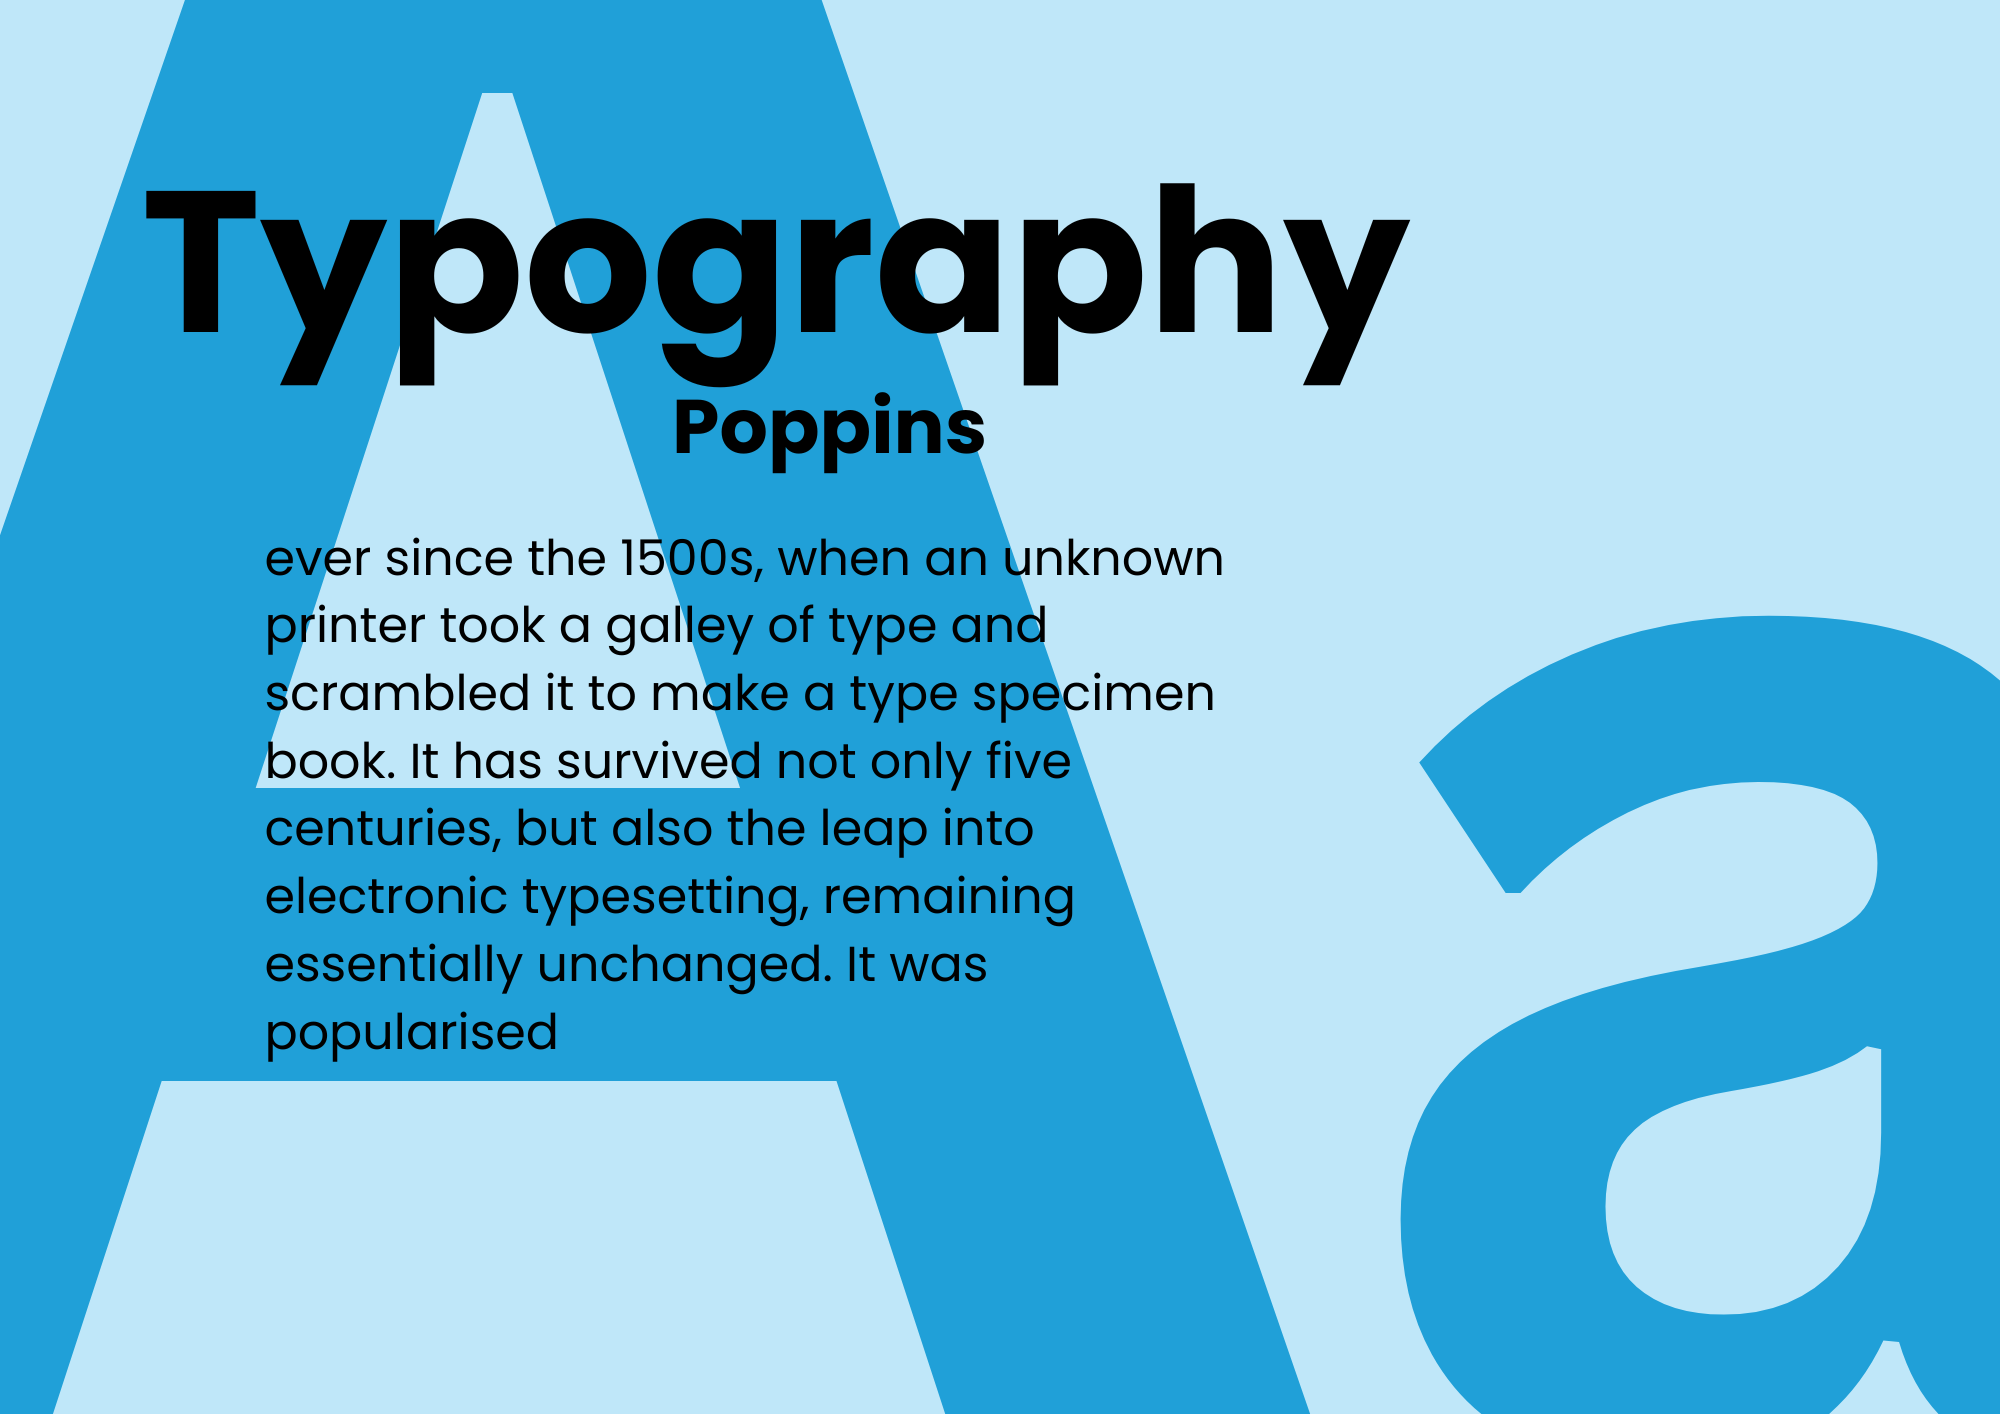
\includegraphics[width=0.7\textwidth]{images/1.png}
    \caption{Typography (Poppins)}
    \label{fig:figure4}
\end{figure}






\section{ Application Interfaces}







\begin{figure}[H]
	\hspace{1cm}
	\begin {minipage}[t]{4cm}
	\centering
	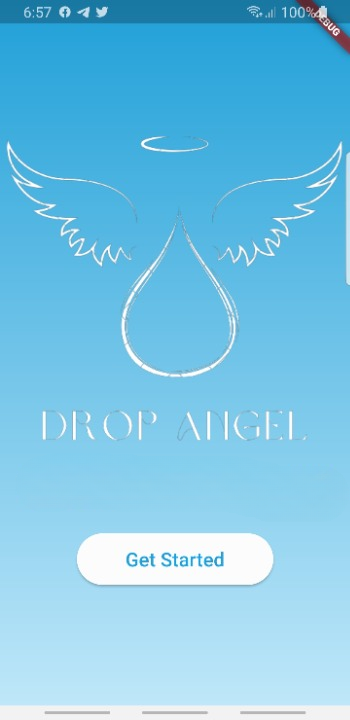
\includegraphics [ width =6 cm ]{images1/welcom_cleanup.jpg}
	\end {minipage}
	\hspace{2.5cm}
	\begin {minipage}[t]{4cm}
	\raggedright
	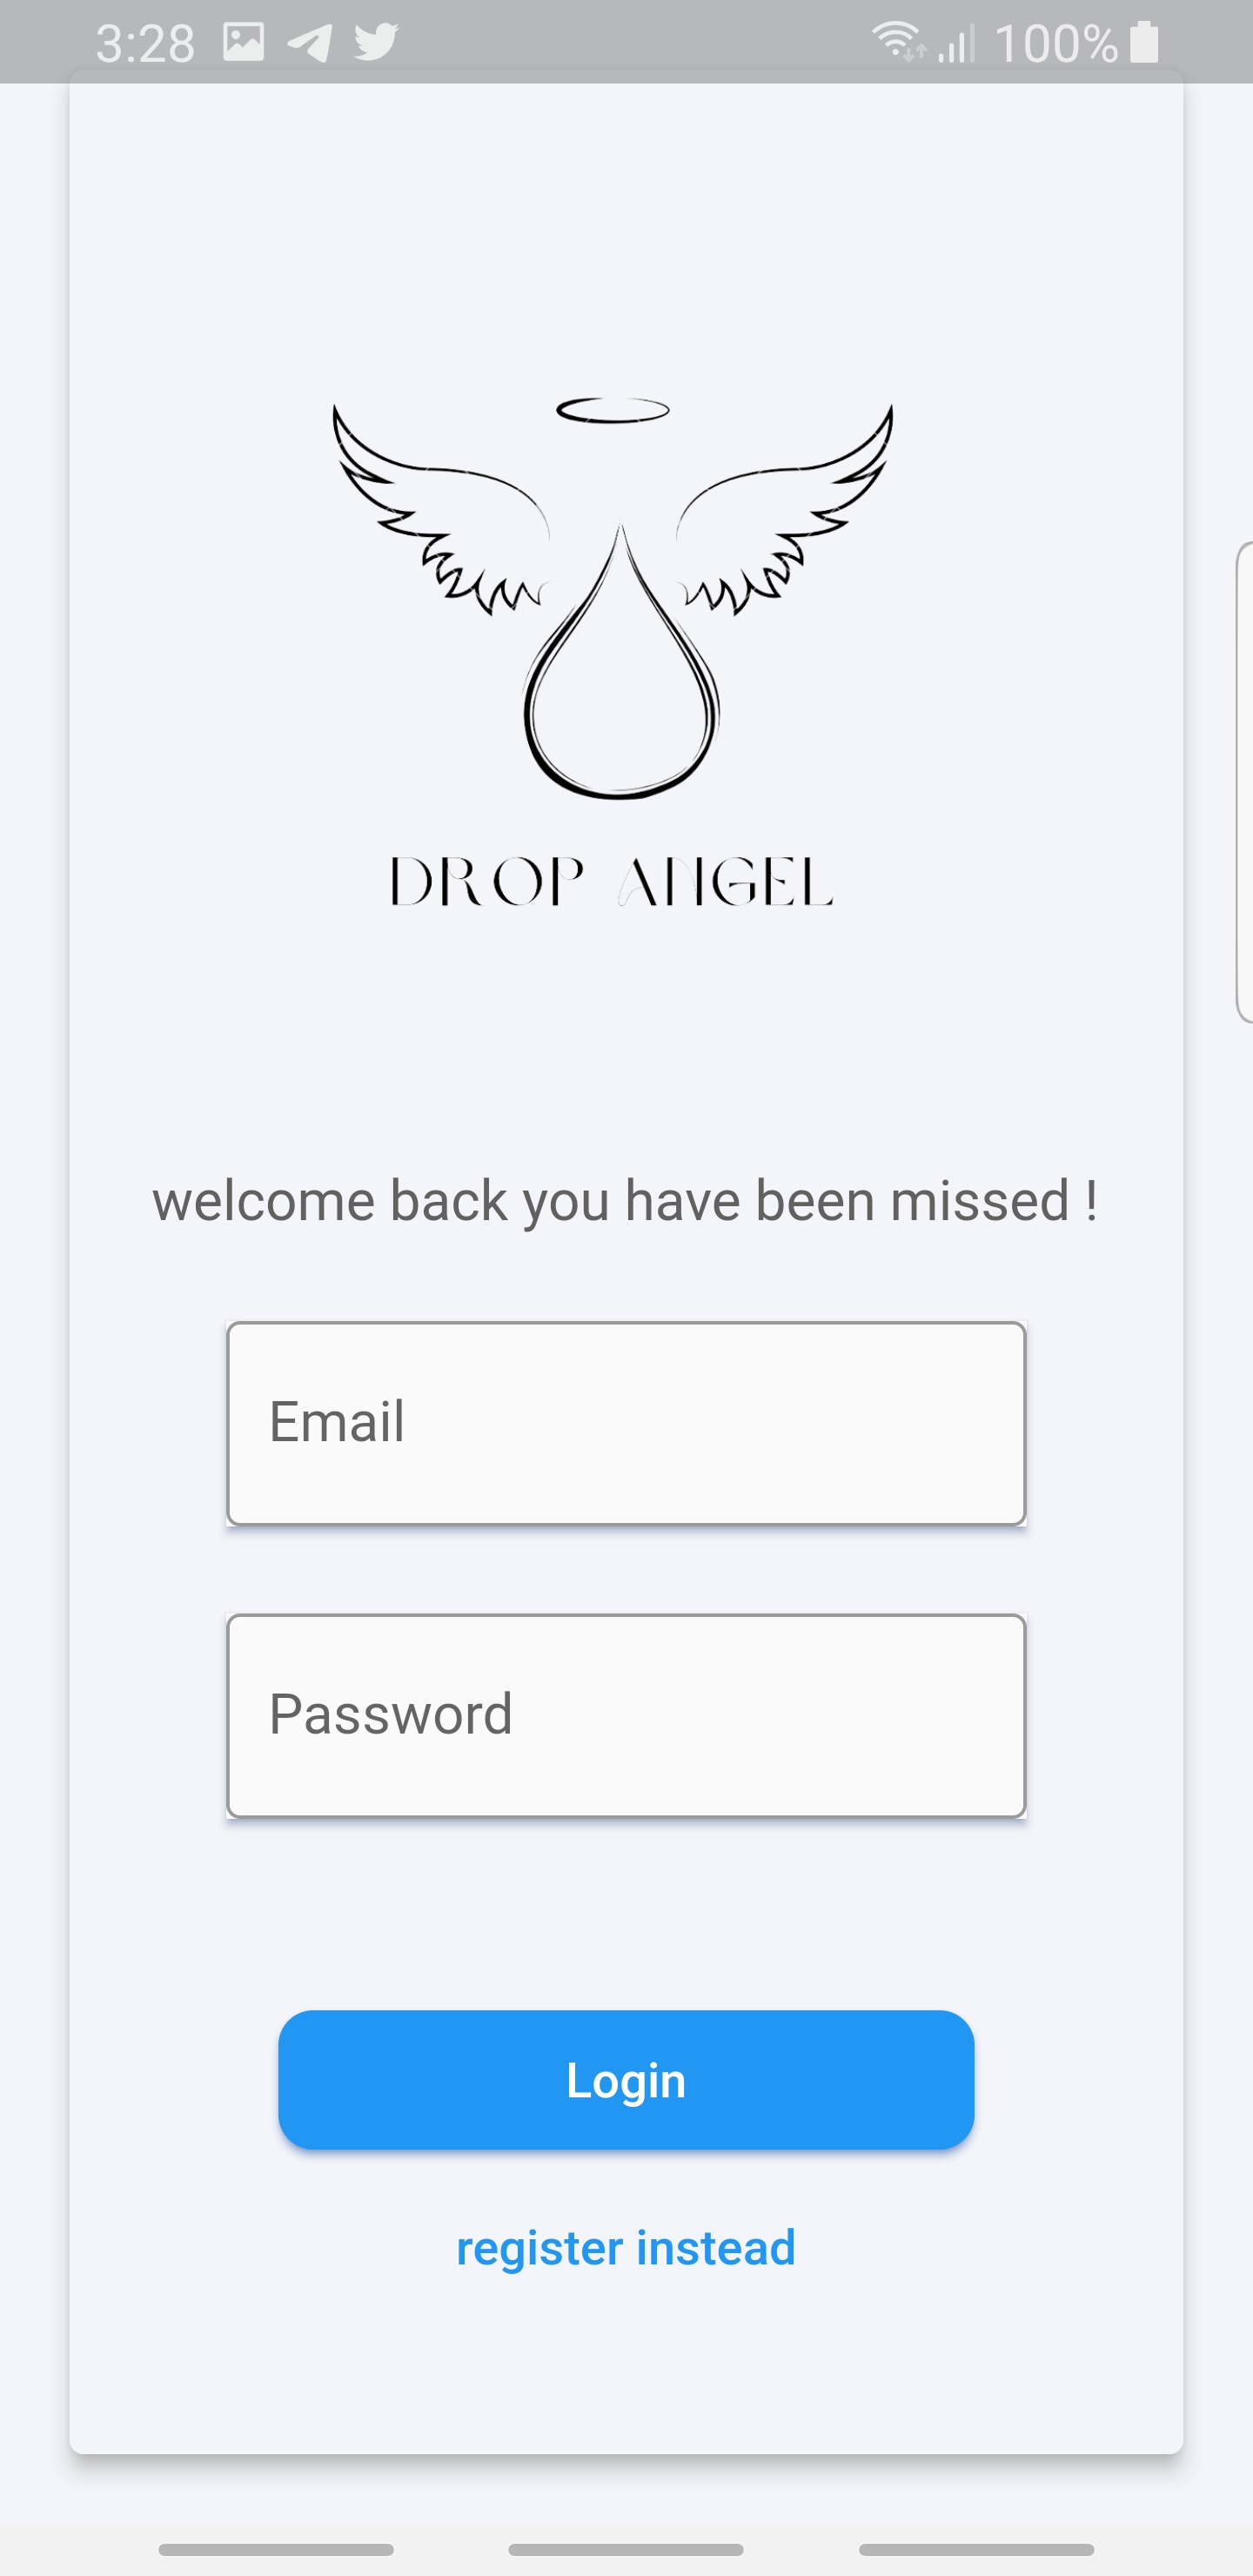
\includegraphics [ width =6 cm ]{images1/login.jpg}
	\end {minipage}
	\caption{Start pages}
\end{figure}




\begin{figure}[H]
	\hspace{1cm}
	\begin {minipage}[t]{4cm}
	\centering
	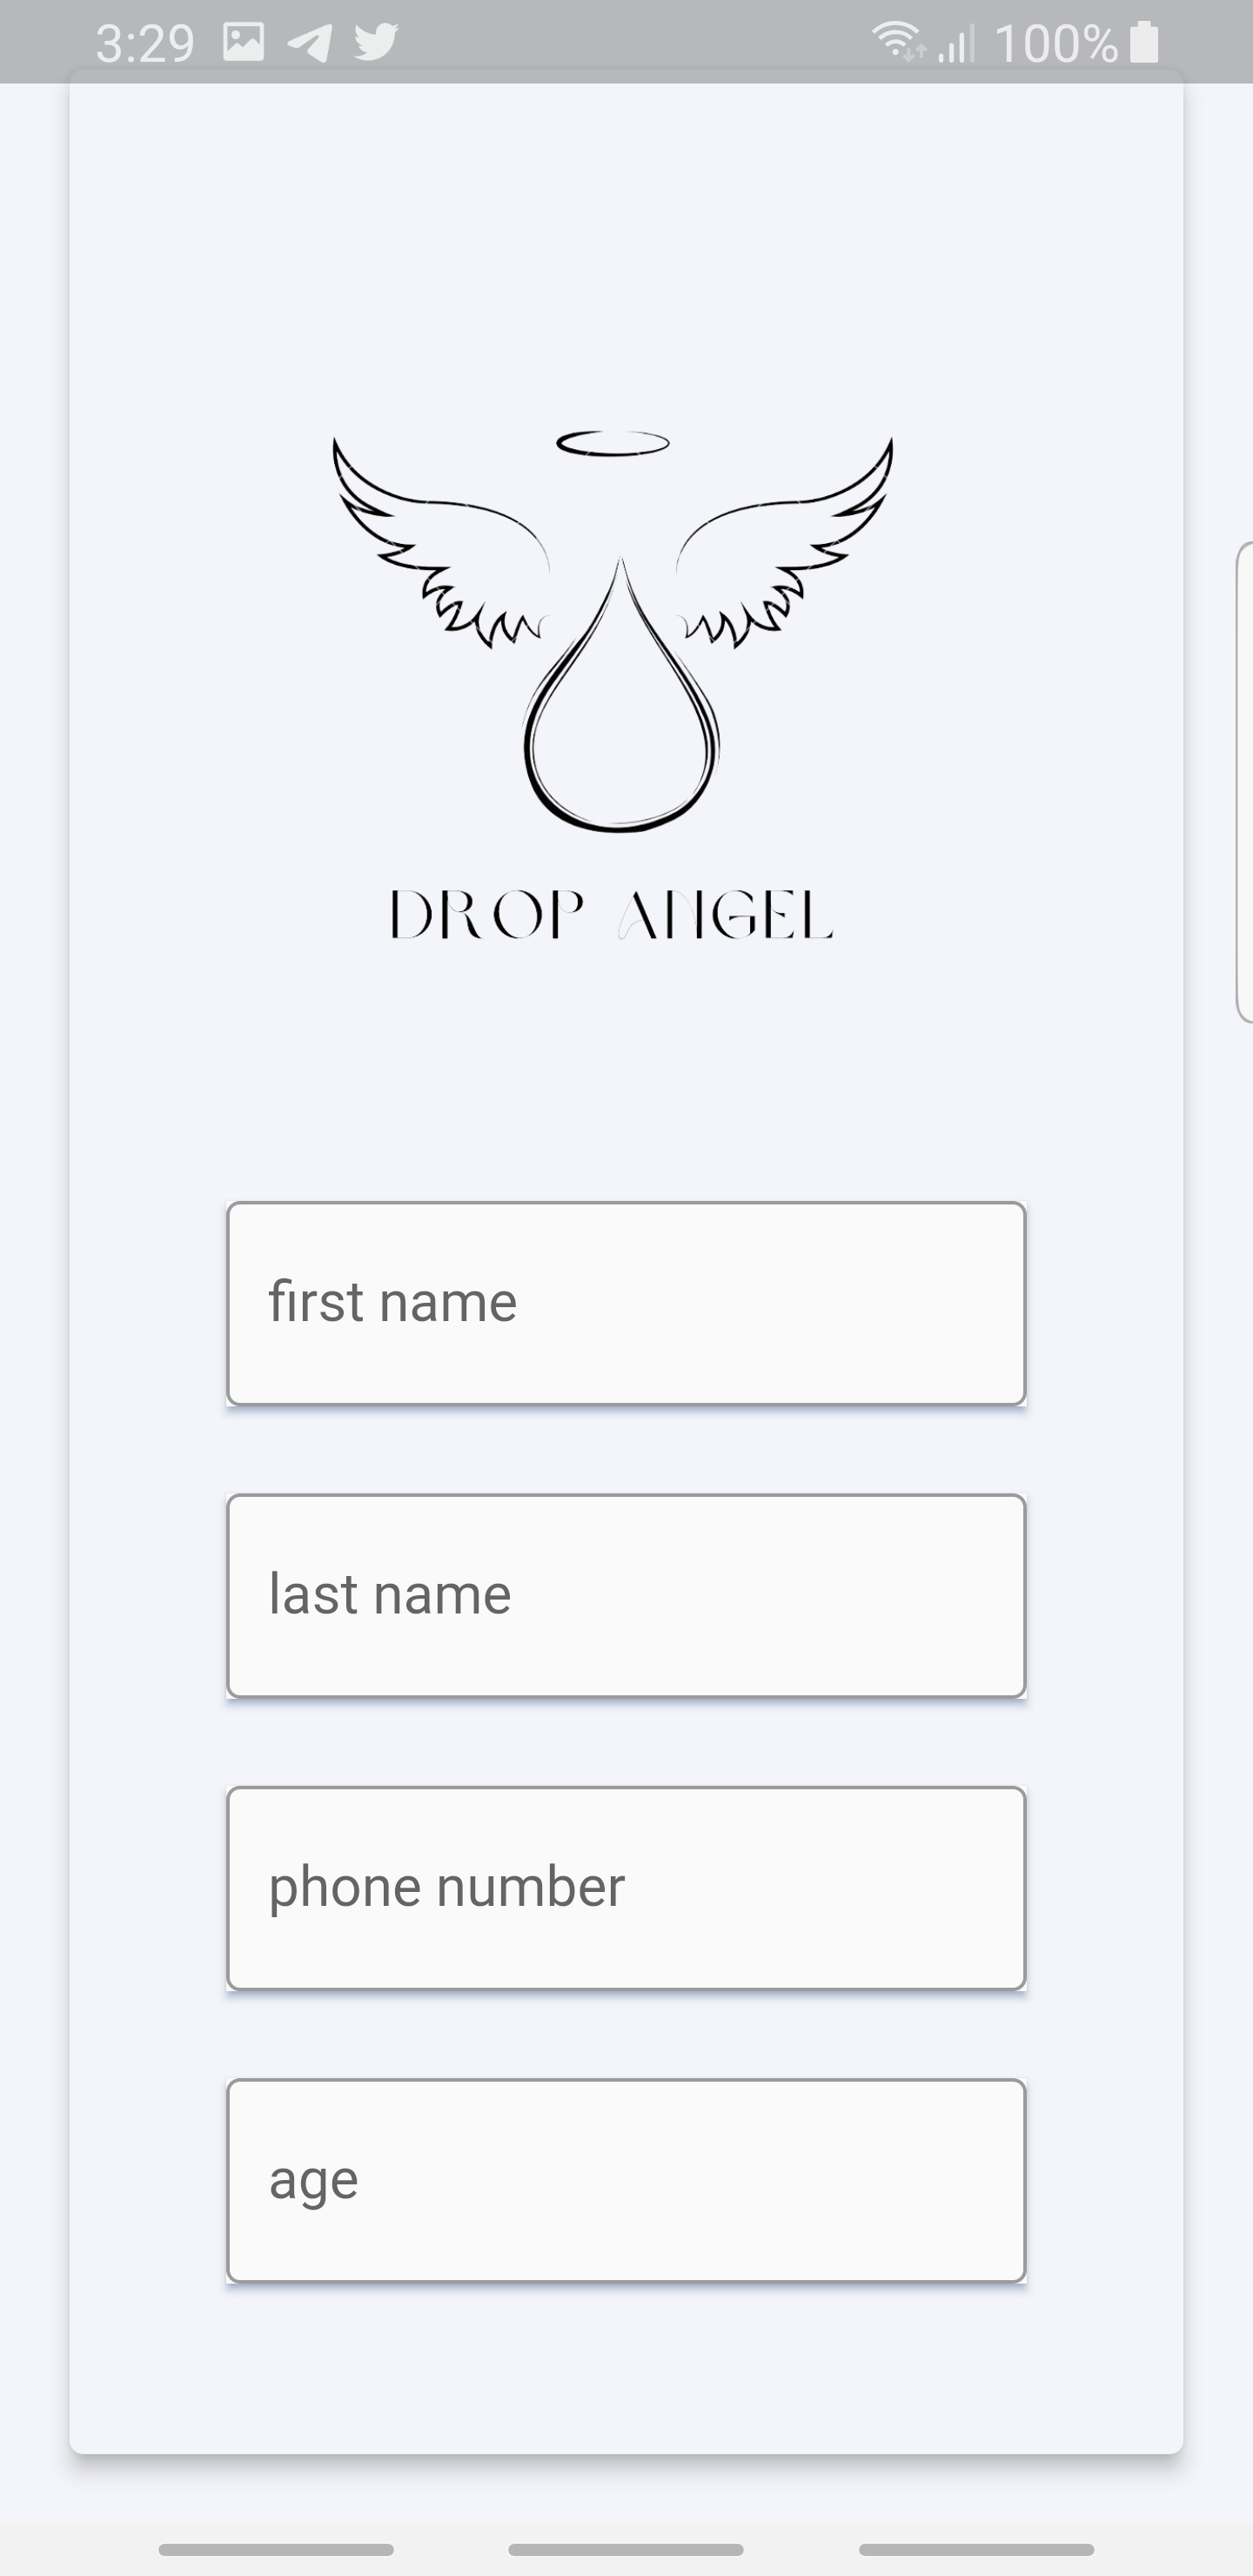
\includegraphics [ width =6 cm ]{images1/register1.jpg}
	\end {minipage}
	\hspace{2.5cm}
	\begin {minipage}[t]{4cm}
	\raggedright
	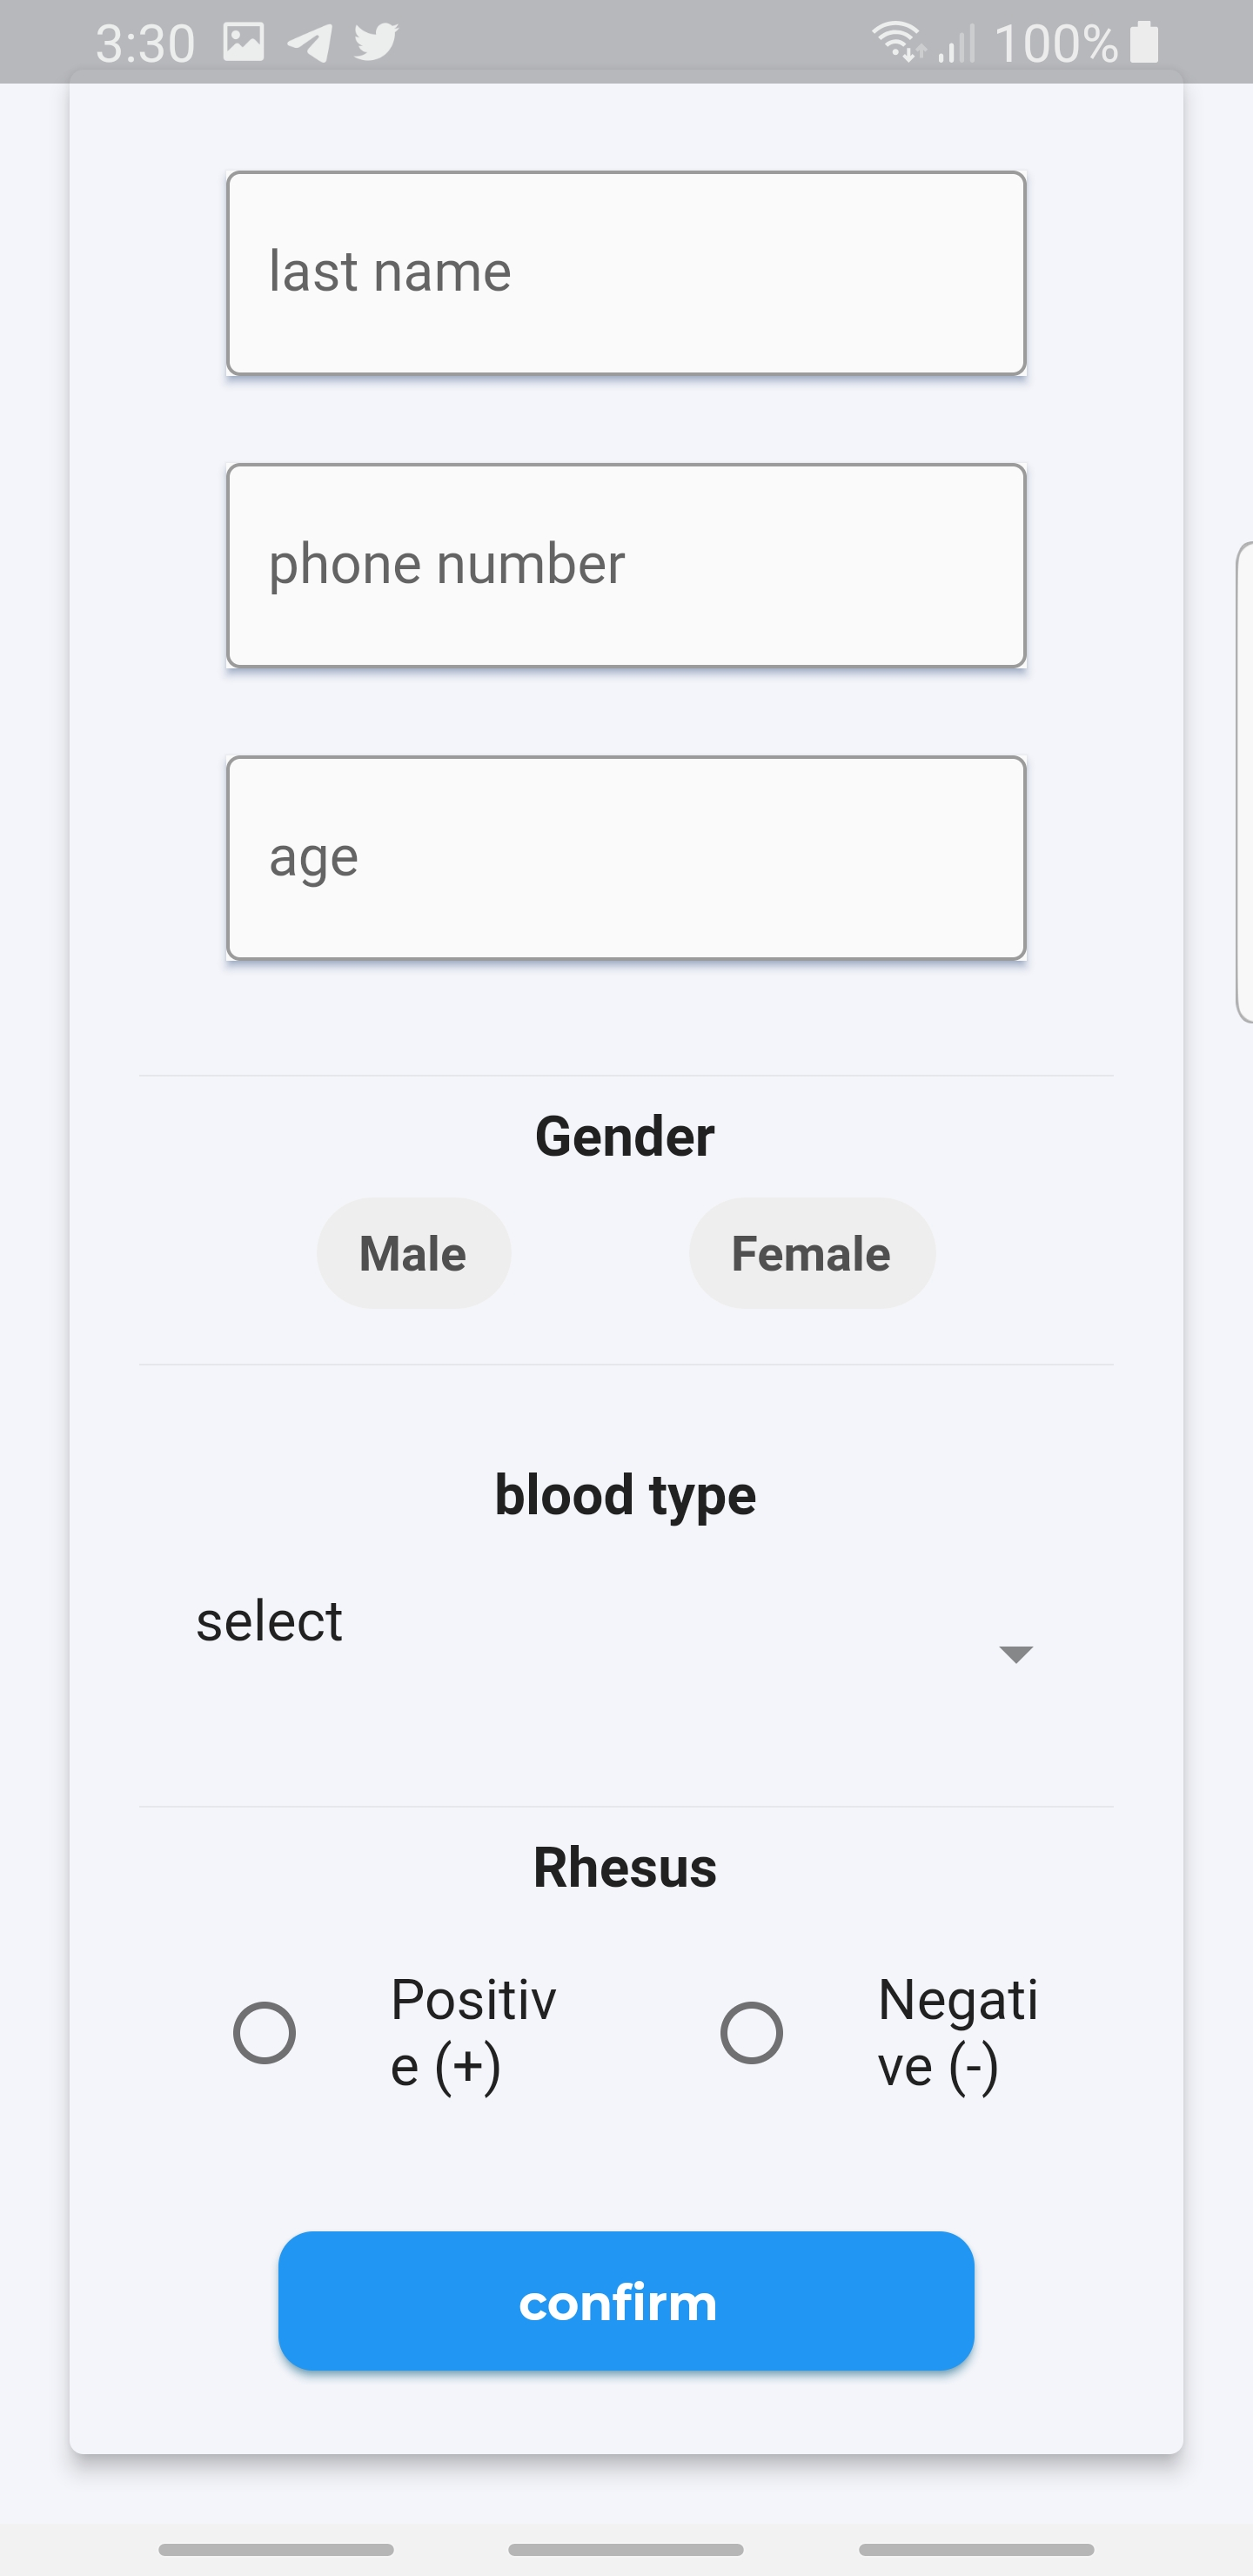
\includegraphics [ width =6 cm ]{images1/register2.jpg}
	\end {minipage}
	\caption{Registration }
\end{figure}


\begin{figure}
\begin{subfigure}{.31\textwidth}
  \centering
  % include first image
  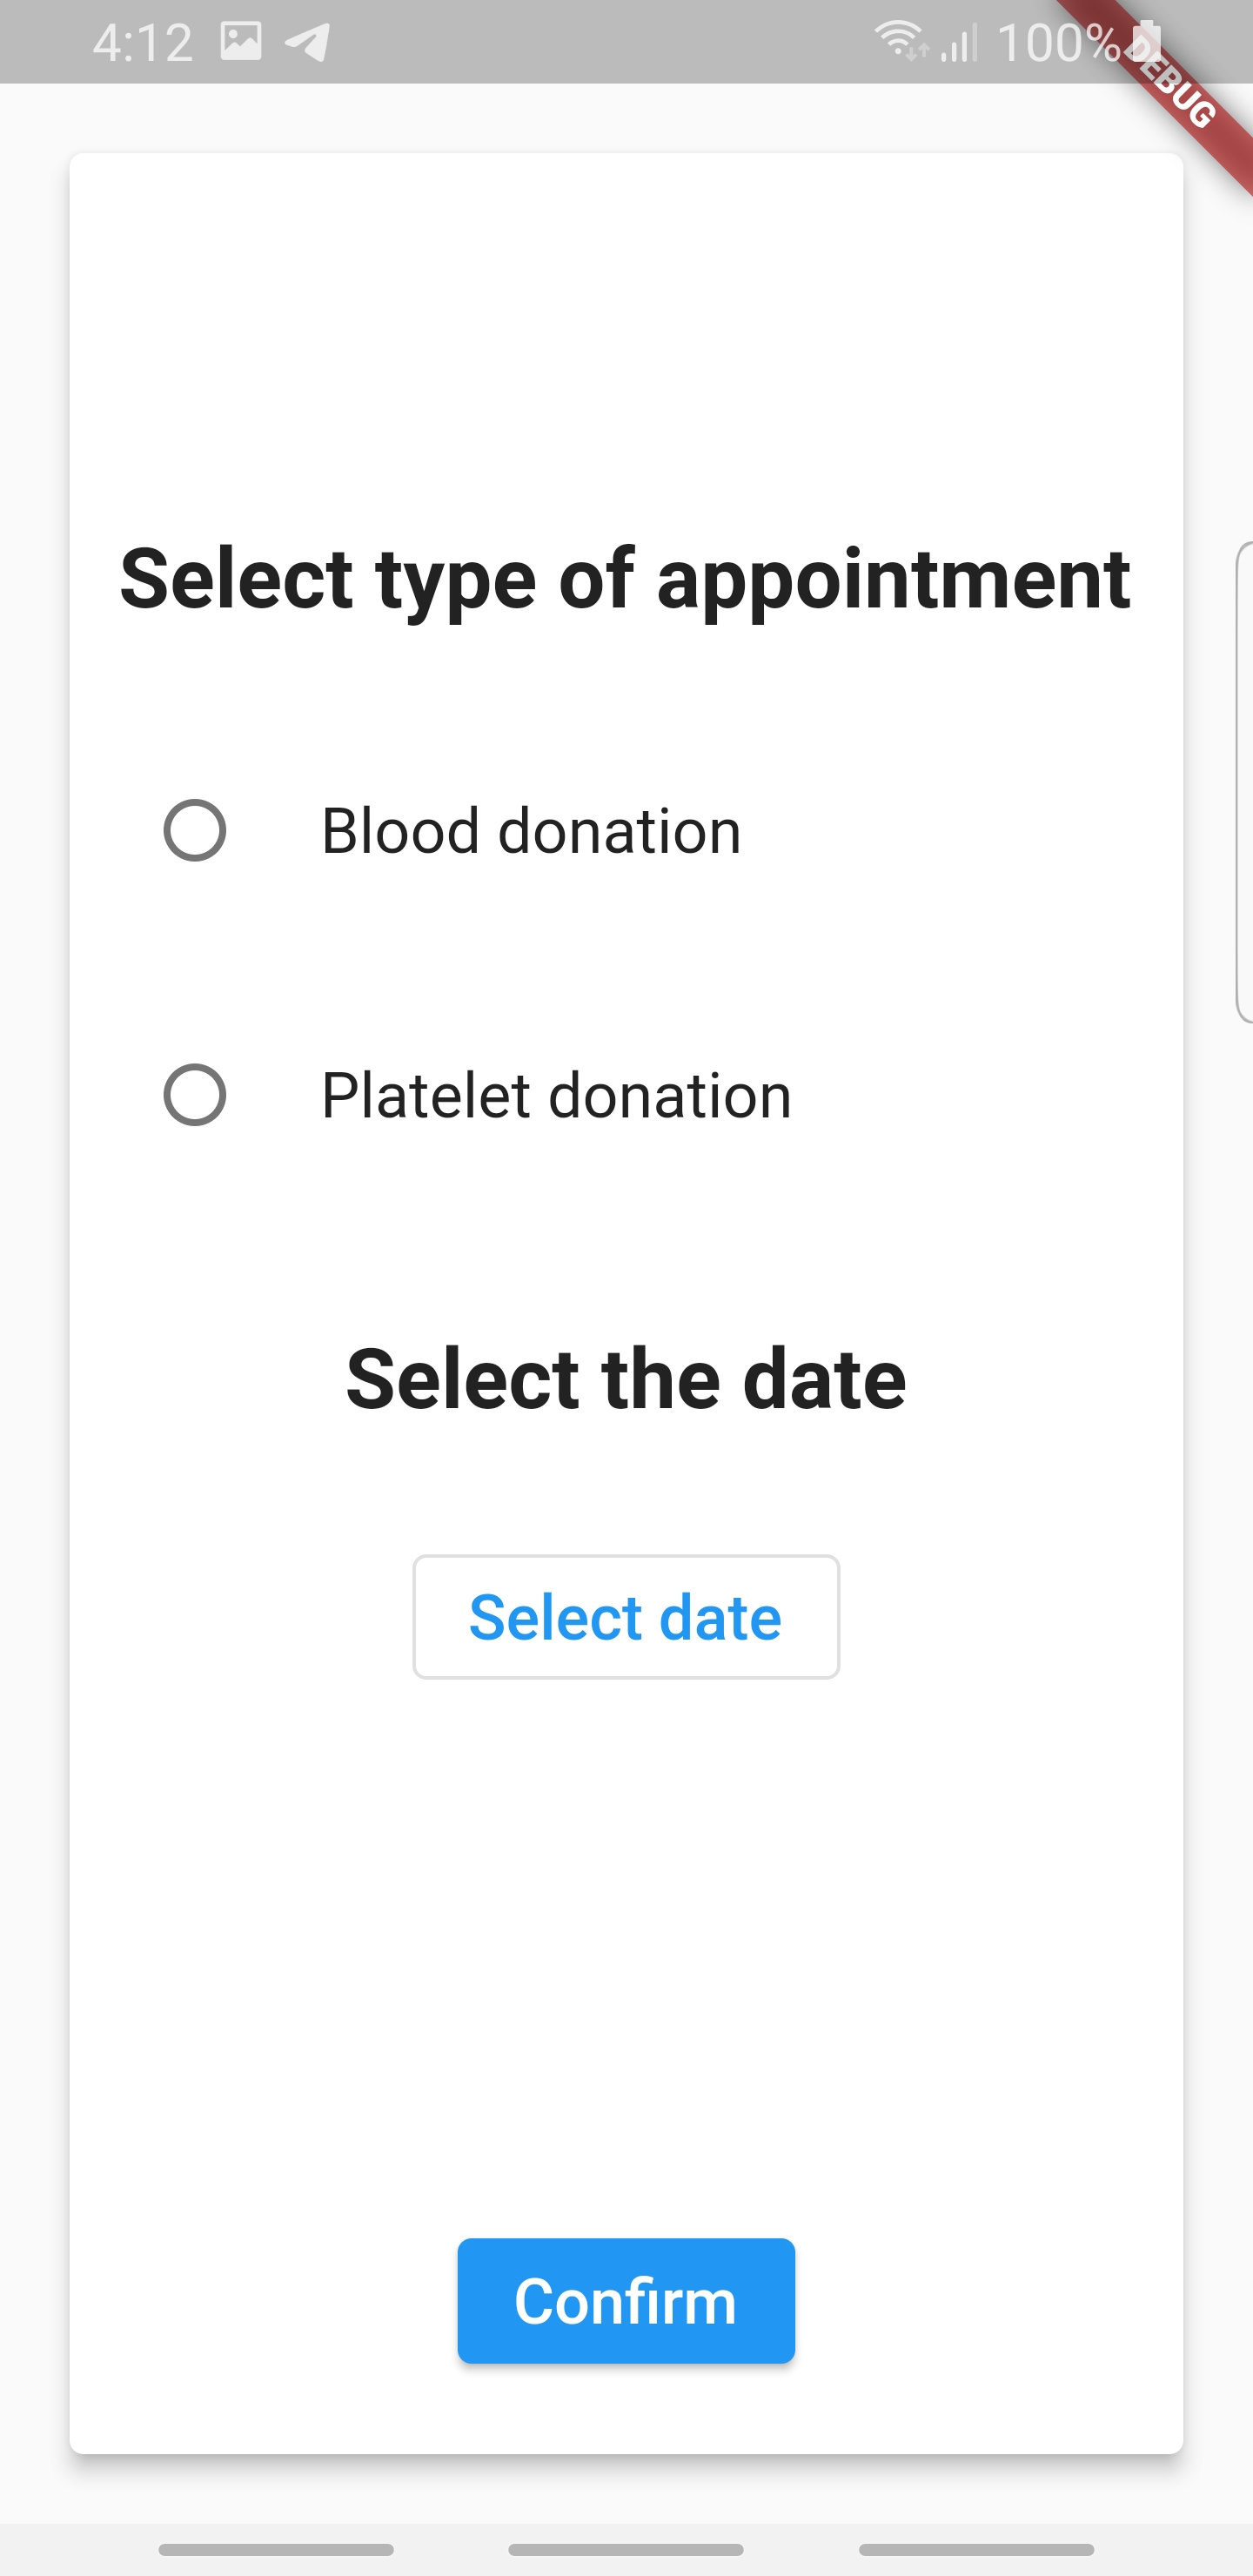
\includegraphics[width=1\linewidth]{images1/quess5.jpg}  
  %\caption{Put your sub-caption here}
  \label{fig:sub-first}
\end{subfigure}
\begin{subfigure}{.31\textwidth}
  \centering
  % include second image
  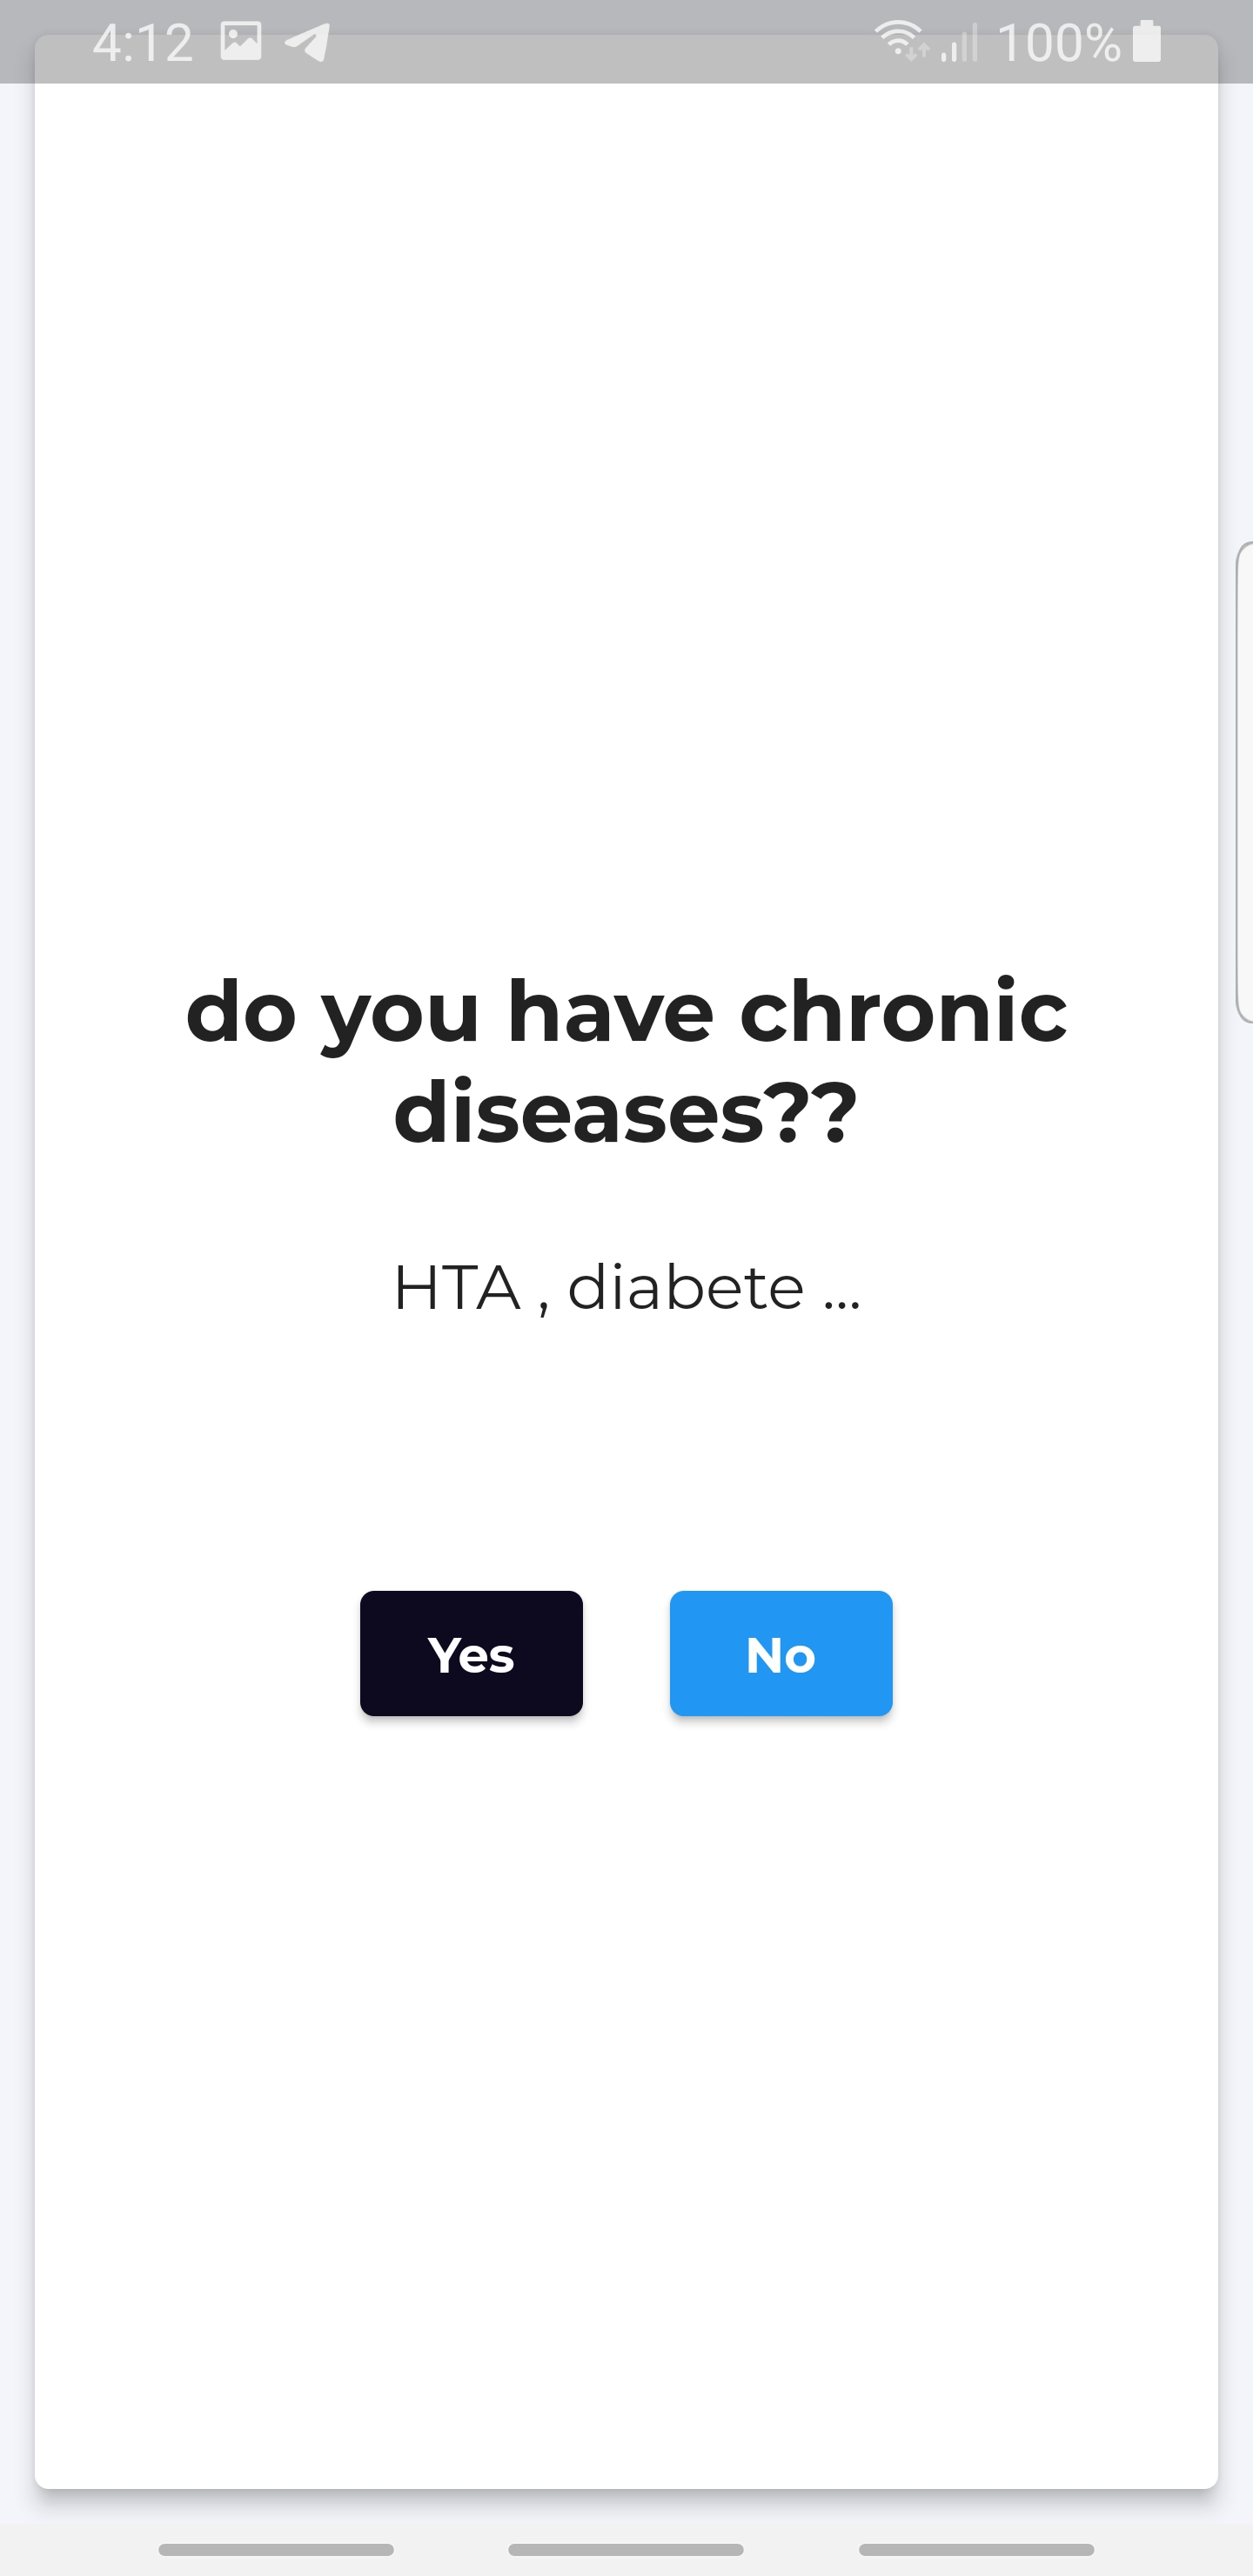
\includegraphics[width=1\linewidth]{images1/quess2.jpg}  
  %\caption{Put your sub-caption here}
  \label{fig:sub-second}
\end{subfigure}
\begin{subfigure}{.31\textwidth}
  \centering
  % include third image
  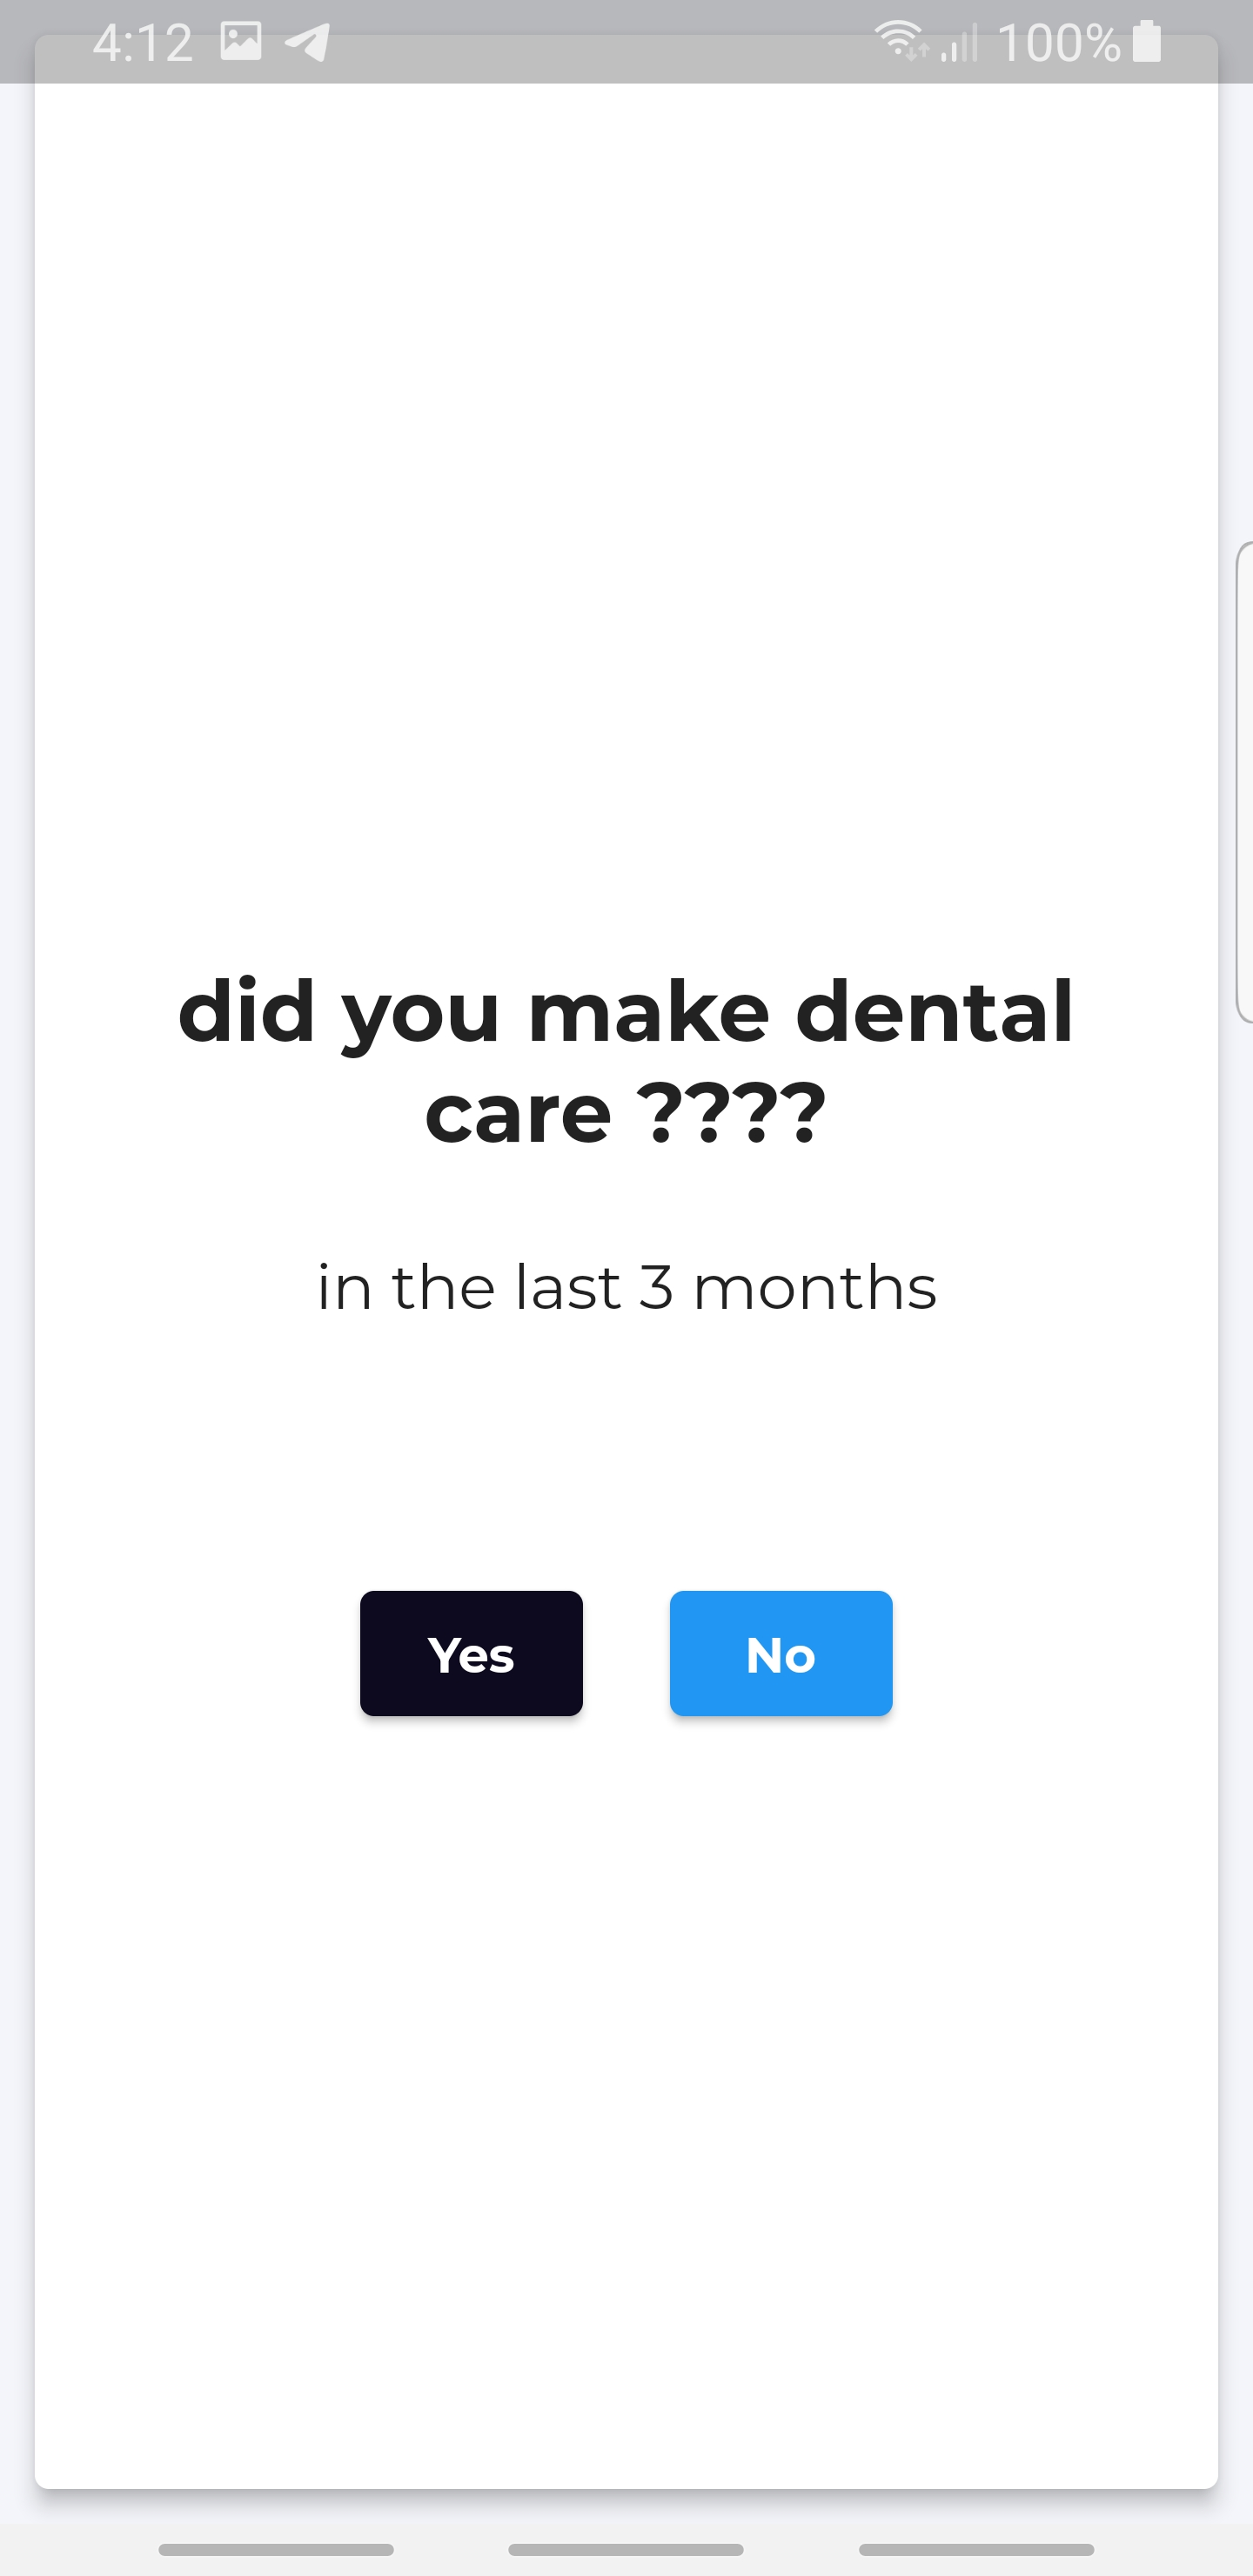
\includegraphics[width=1\linewidth]{images1/quess3.jpg}  
  %\caption{Put your sub-caption here}
  \label{fig:sub-third}
\end{subfigure}
\newline
\begin{subfigure}{.31\textwidth}
  \centering
  % include fourth image
  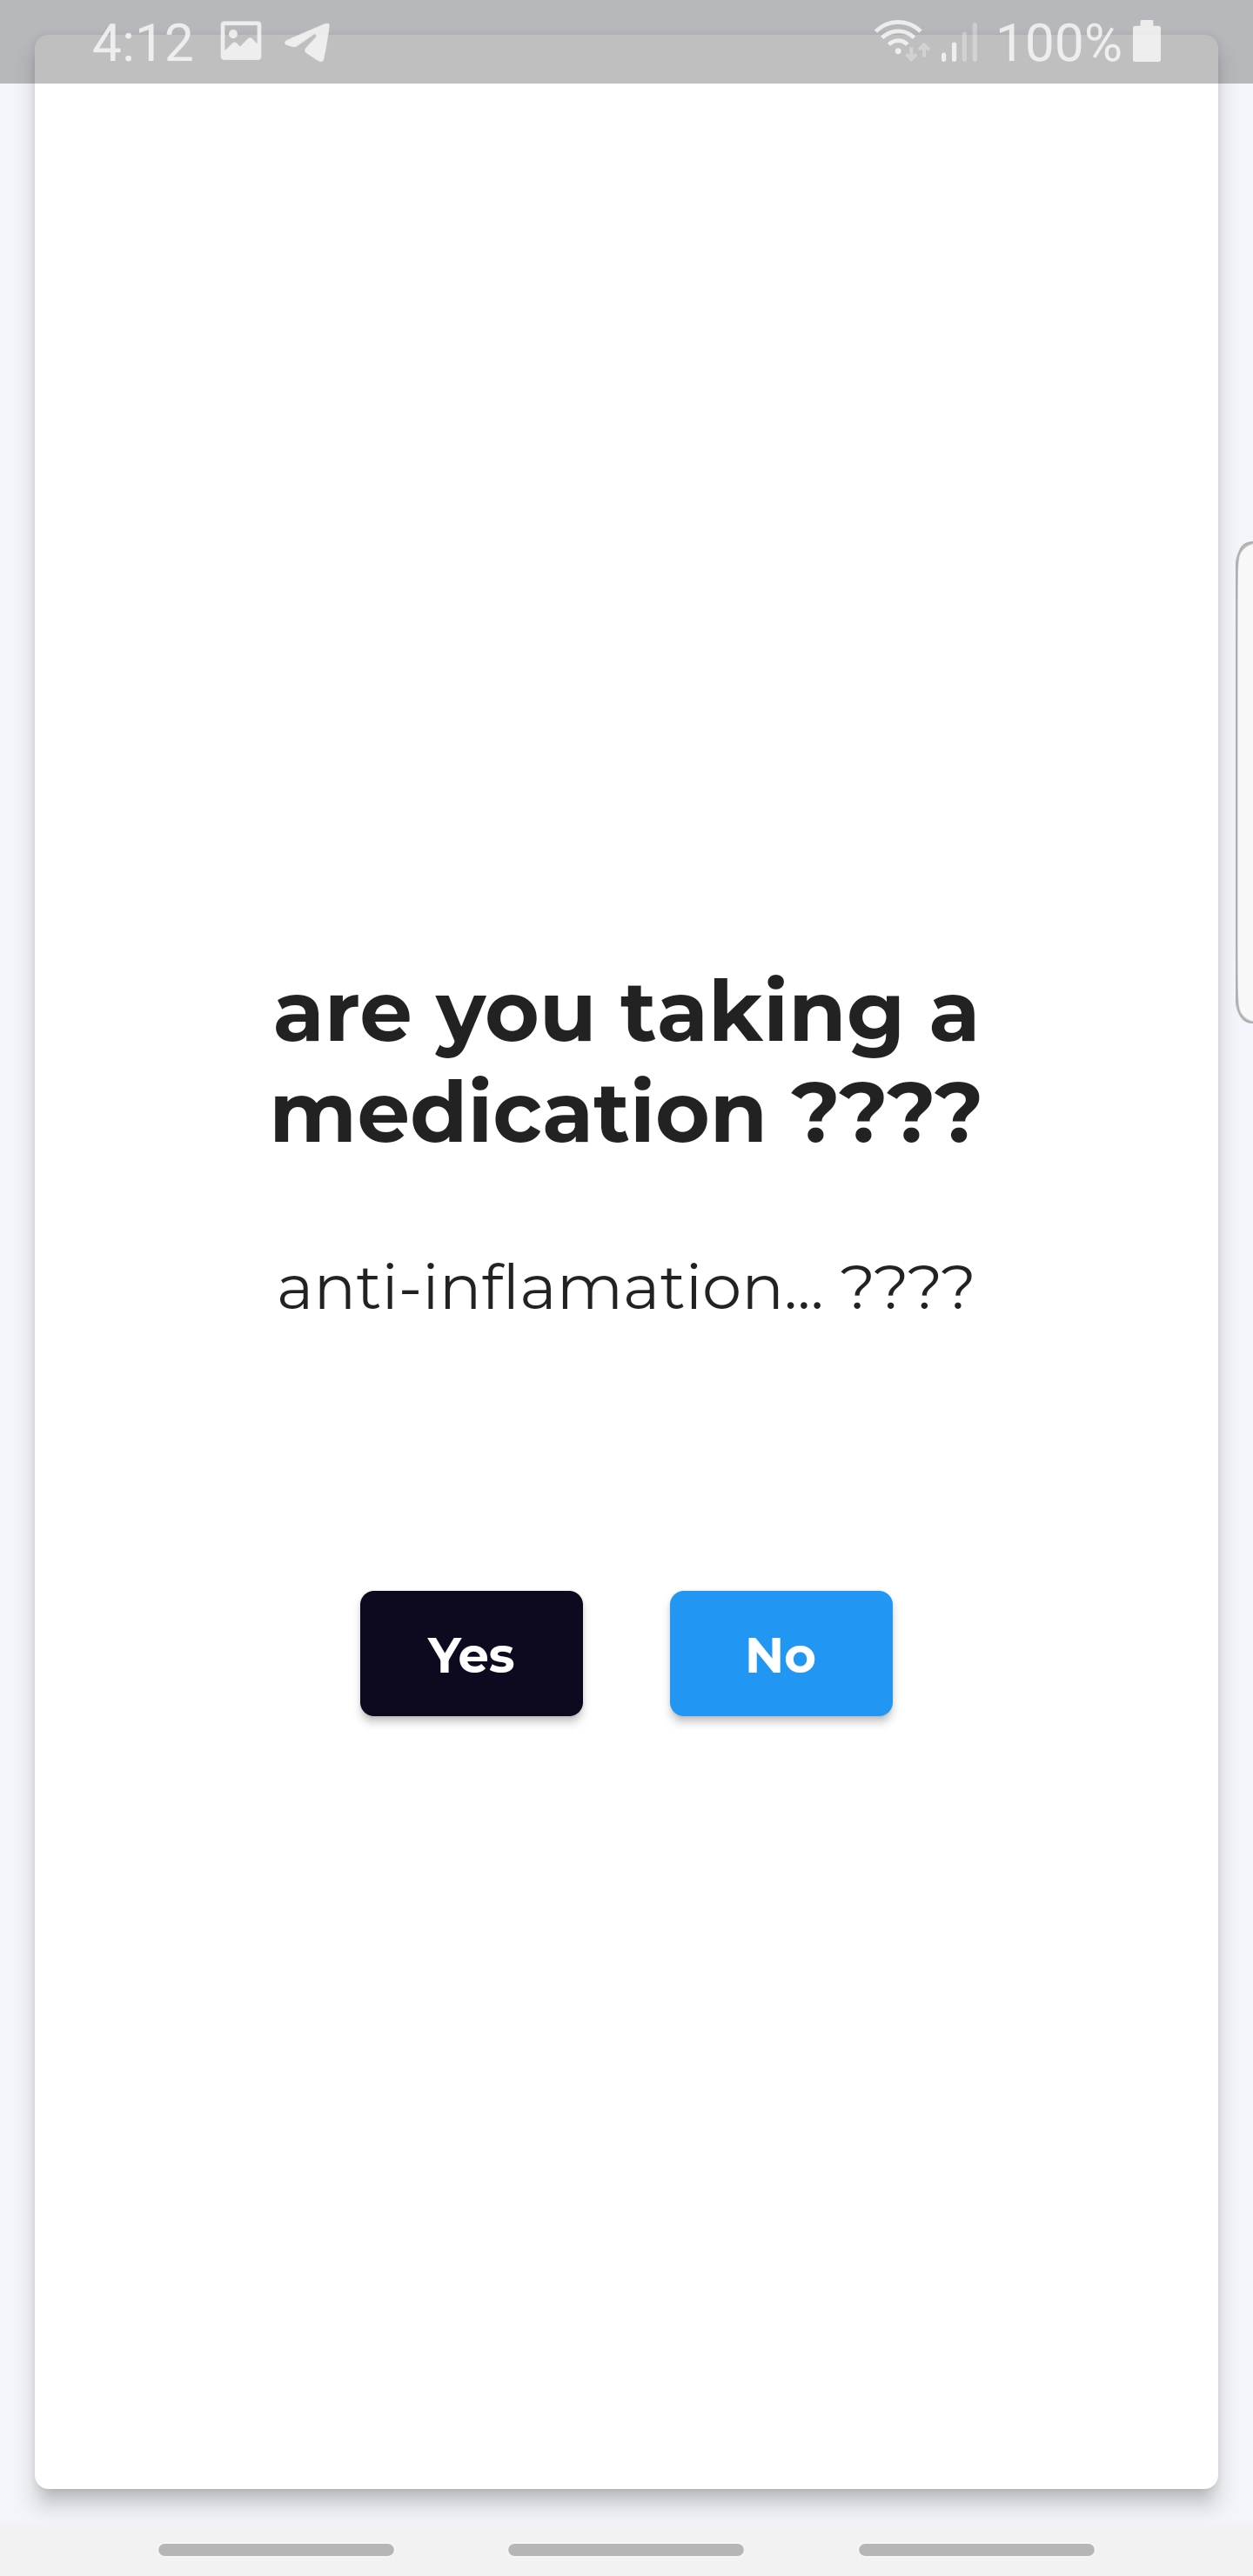
\includegraphics[width=1\linewidth]{images1/quess4.jpg}  
  %\caption{Put your sub-caption here}
  \label{fig:sub-fourth}
\end{subfigure}
\begin{subfigure}{.31\textwidth}
  \centering
  % include first image
  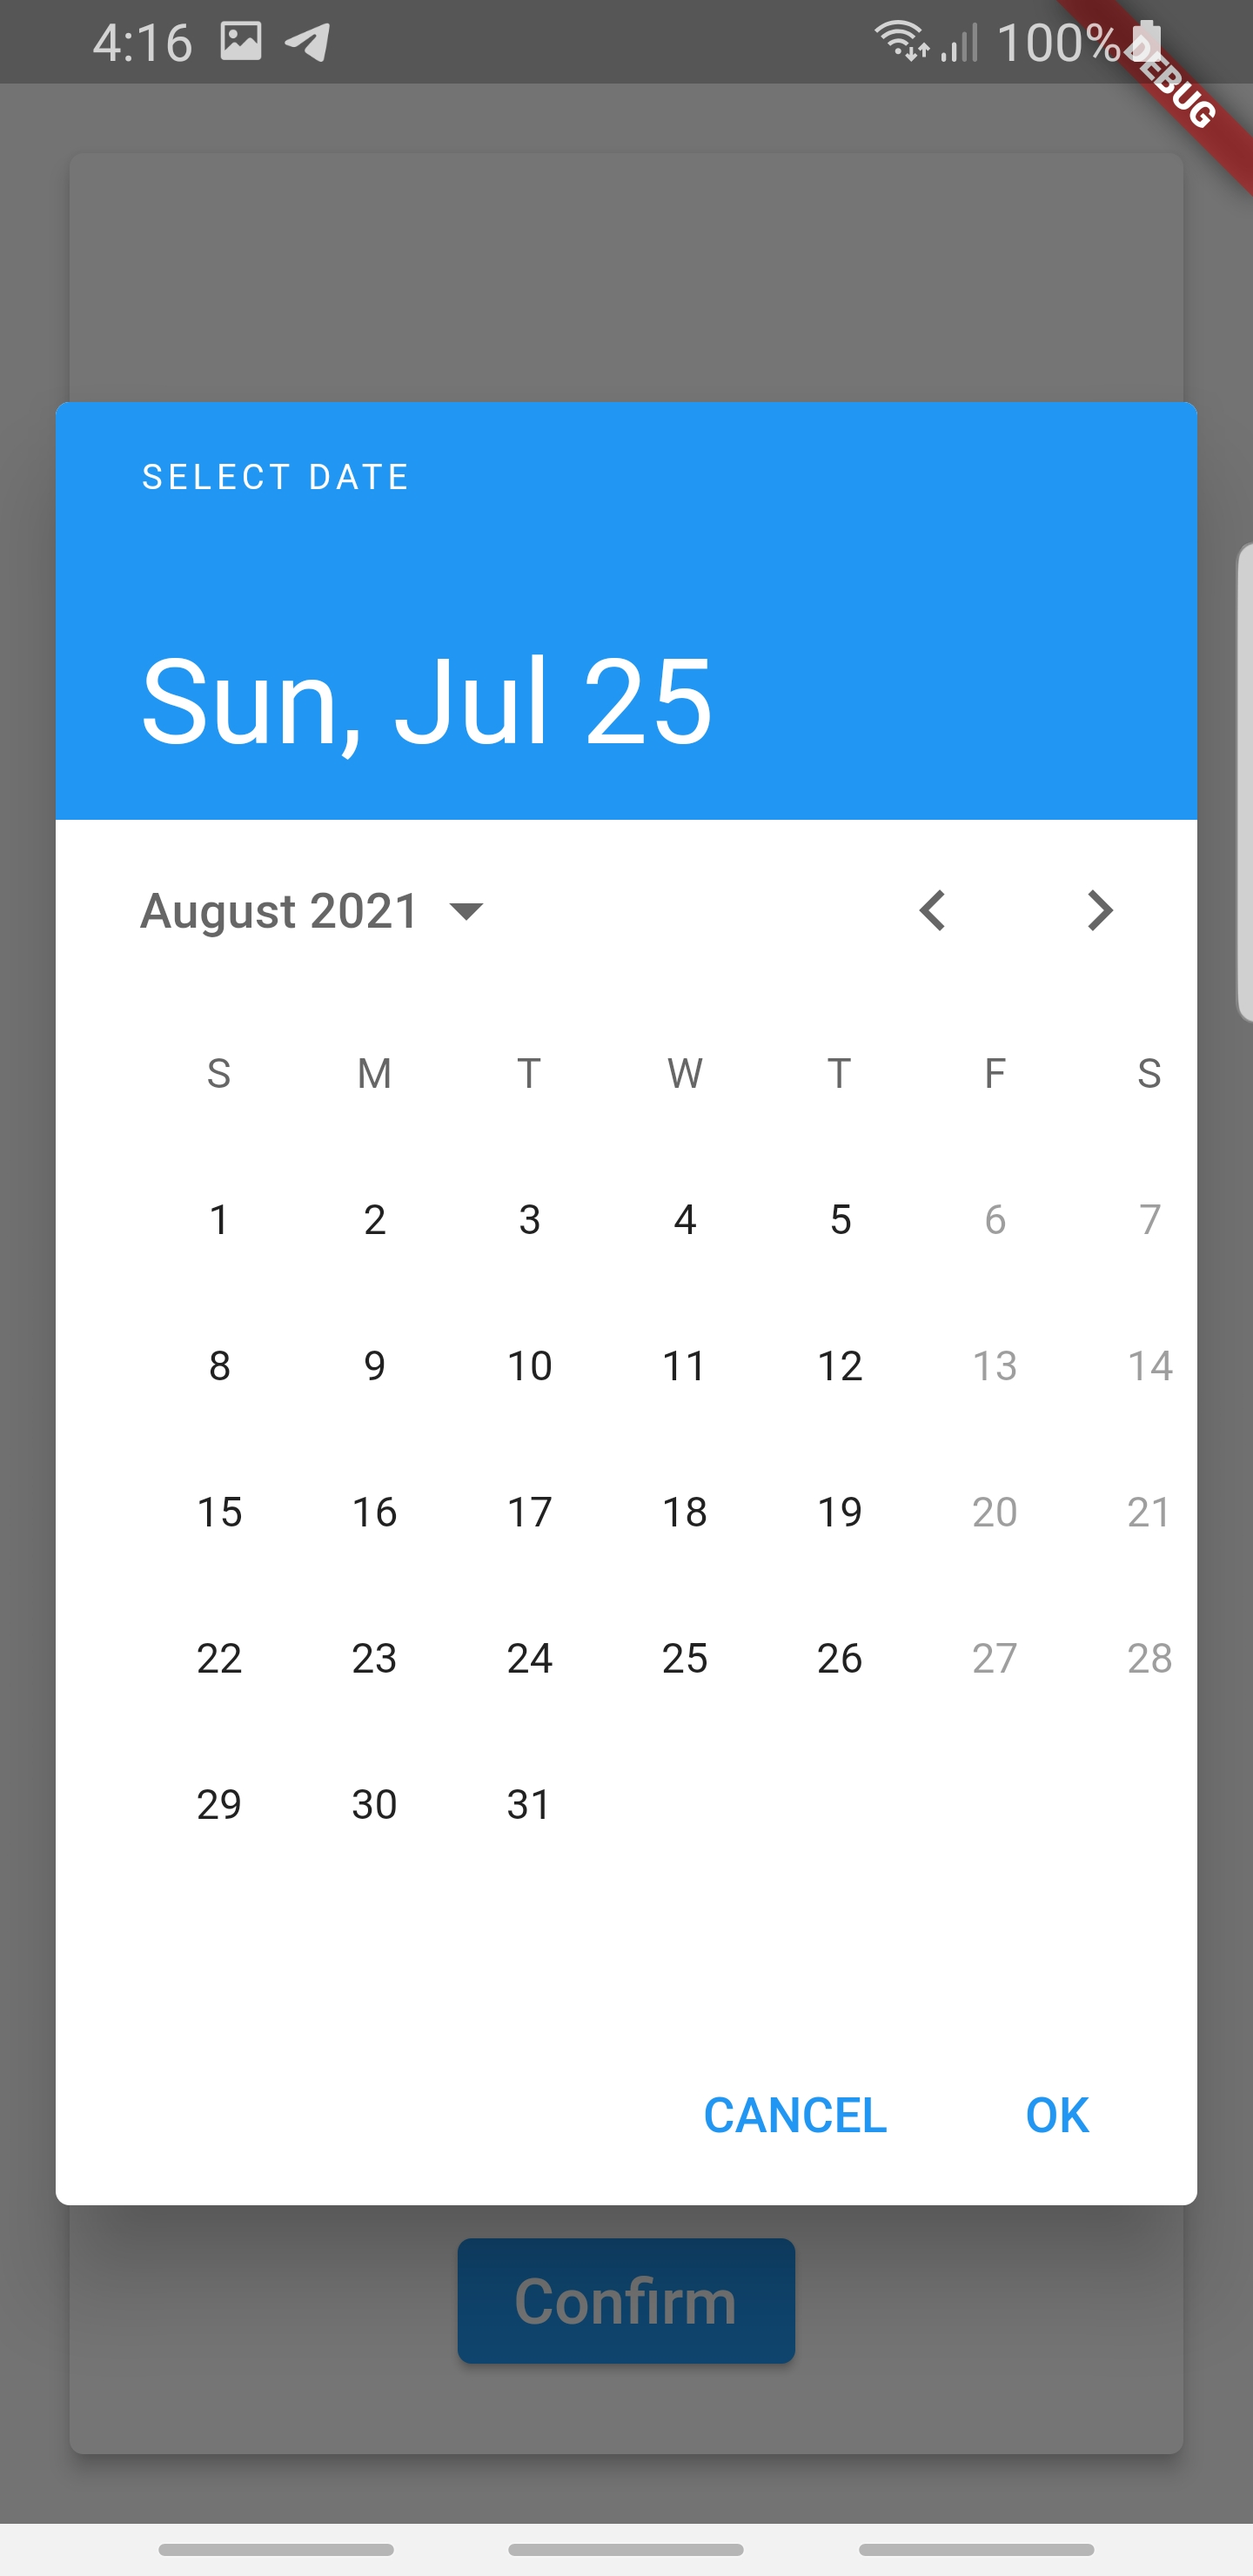
\includegraphics[width=1\linewidth]{images1/ques6.jpg}  
  %\caption{Put your sub-caption here}
  \label{fig:sub-first}
\end{subfigure}
\begin{subfigure}{.31\textwidth}
  \centering
  % include first image
  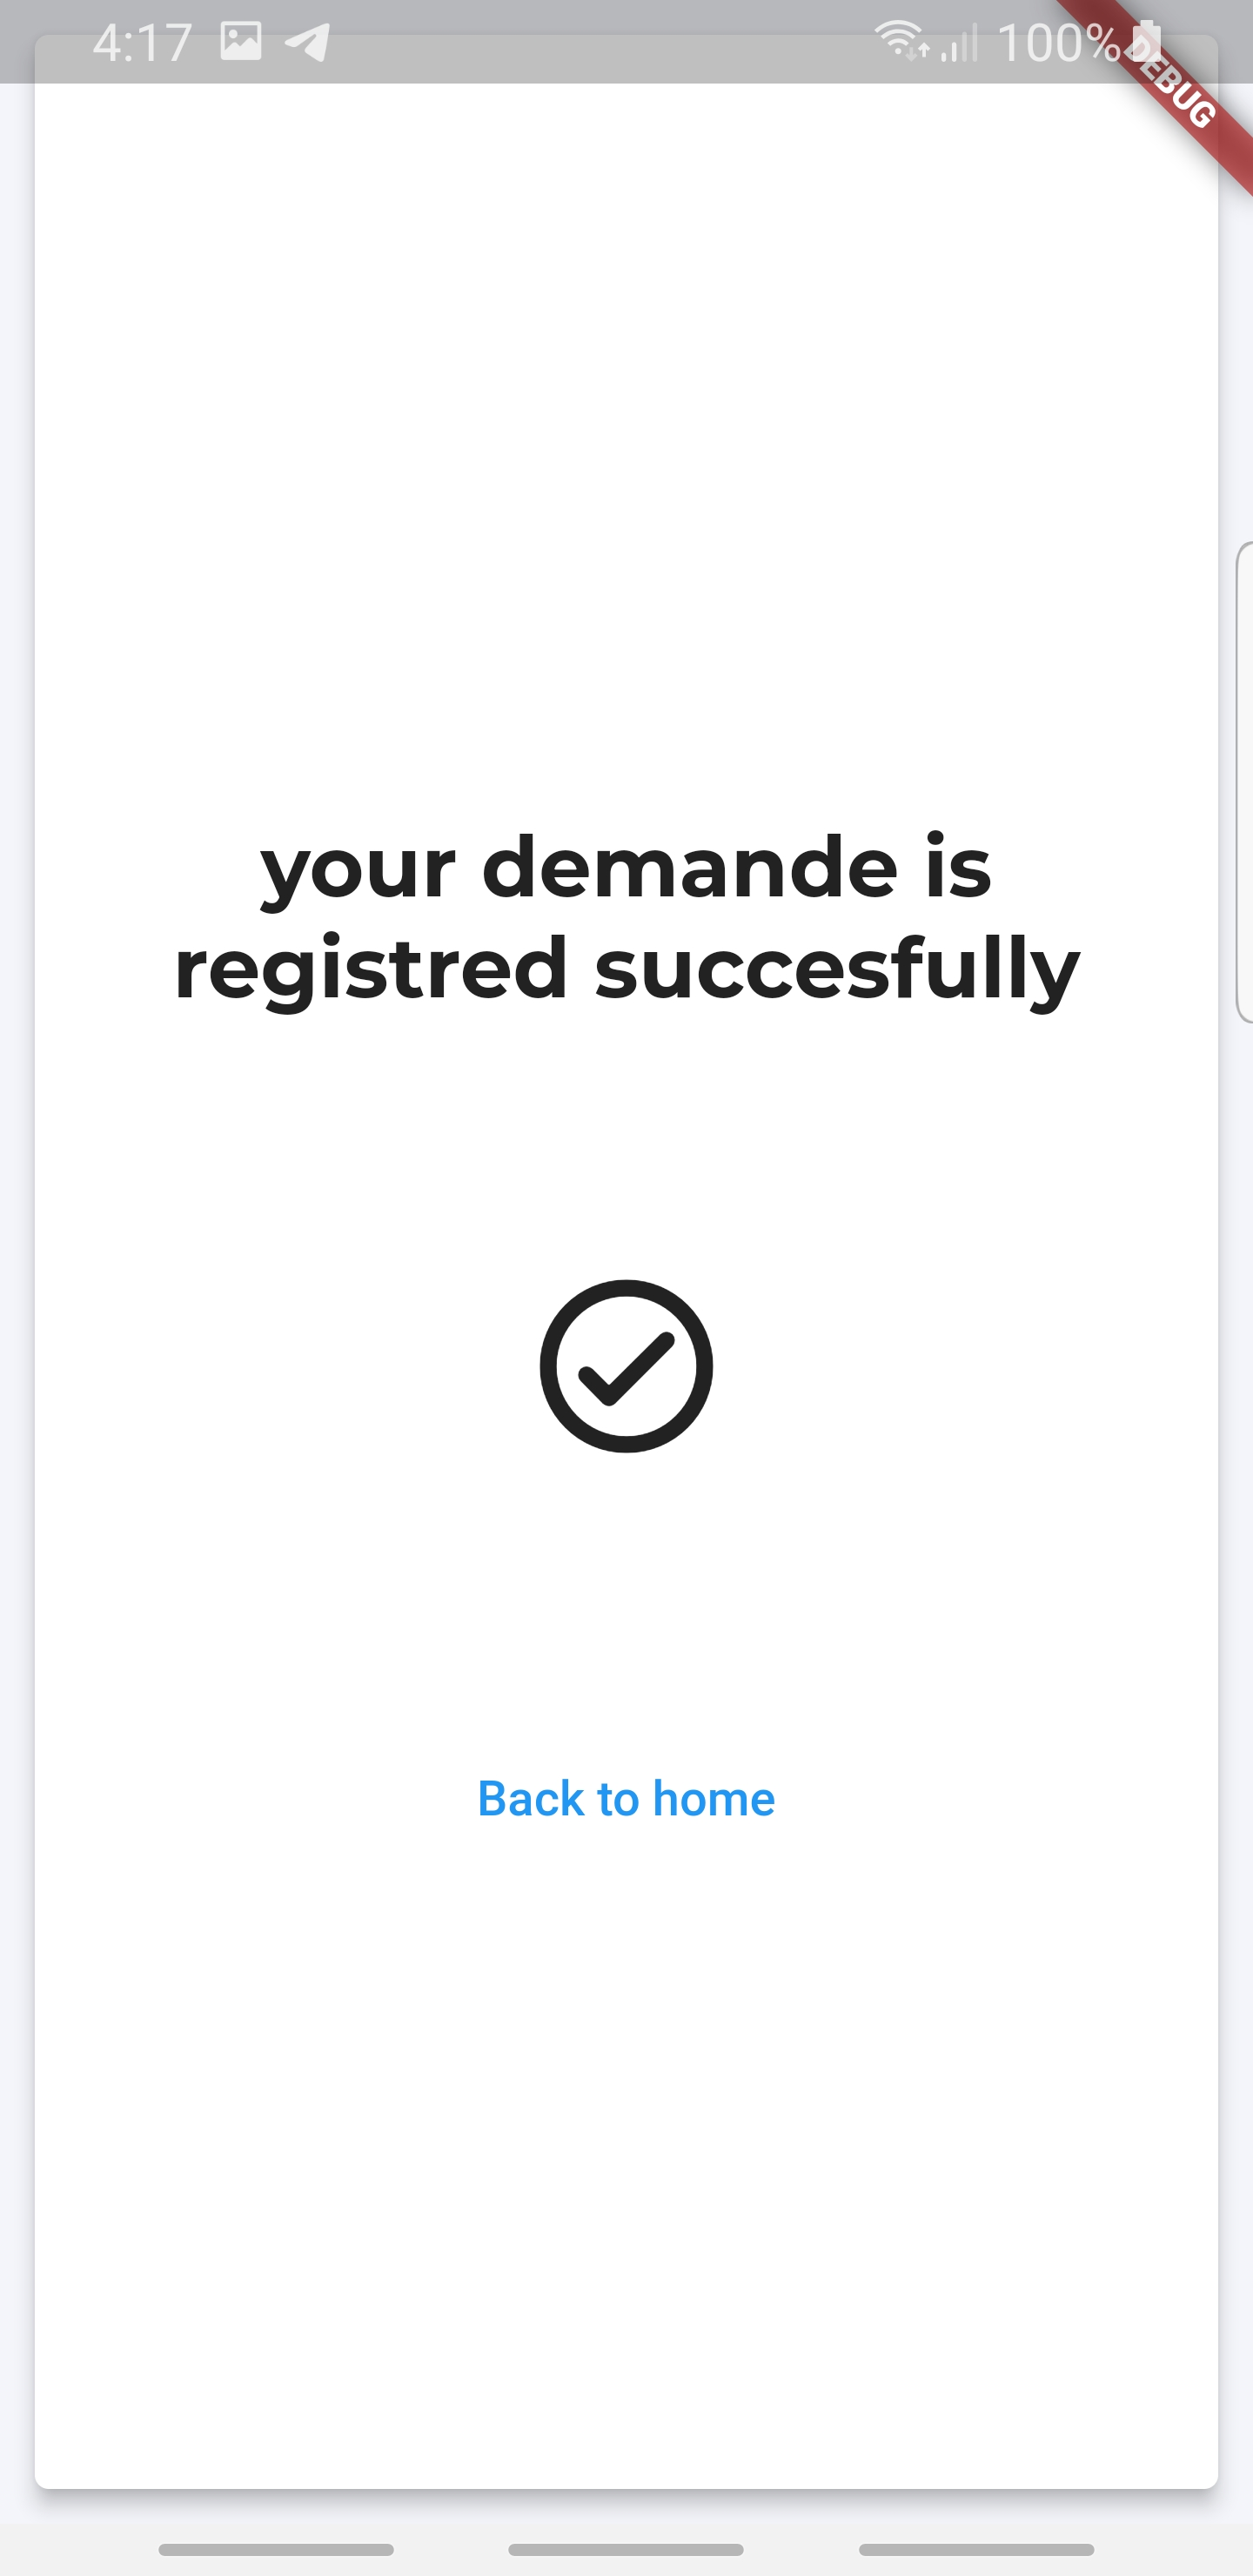
\includegraphics[width=1\linewidth]{images1/ques7.jpg}  
  %\caption{Put your sub-caption here}
  \label{fig:sub-first}
\end{subfigure}
\caption{Registration questions}
\label{fig:fig}
\end{figure}





\begin{figure}[H]
\centering

    \begin{subfigure}[b]{0.409\linewidth}
        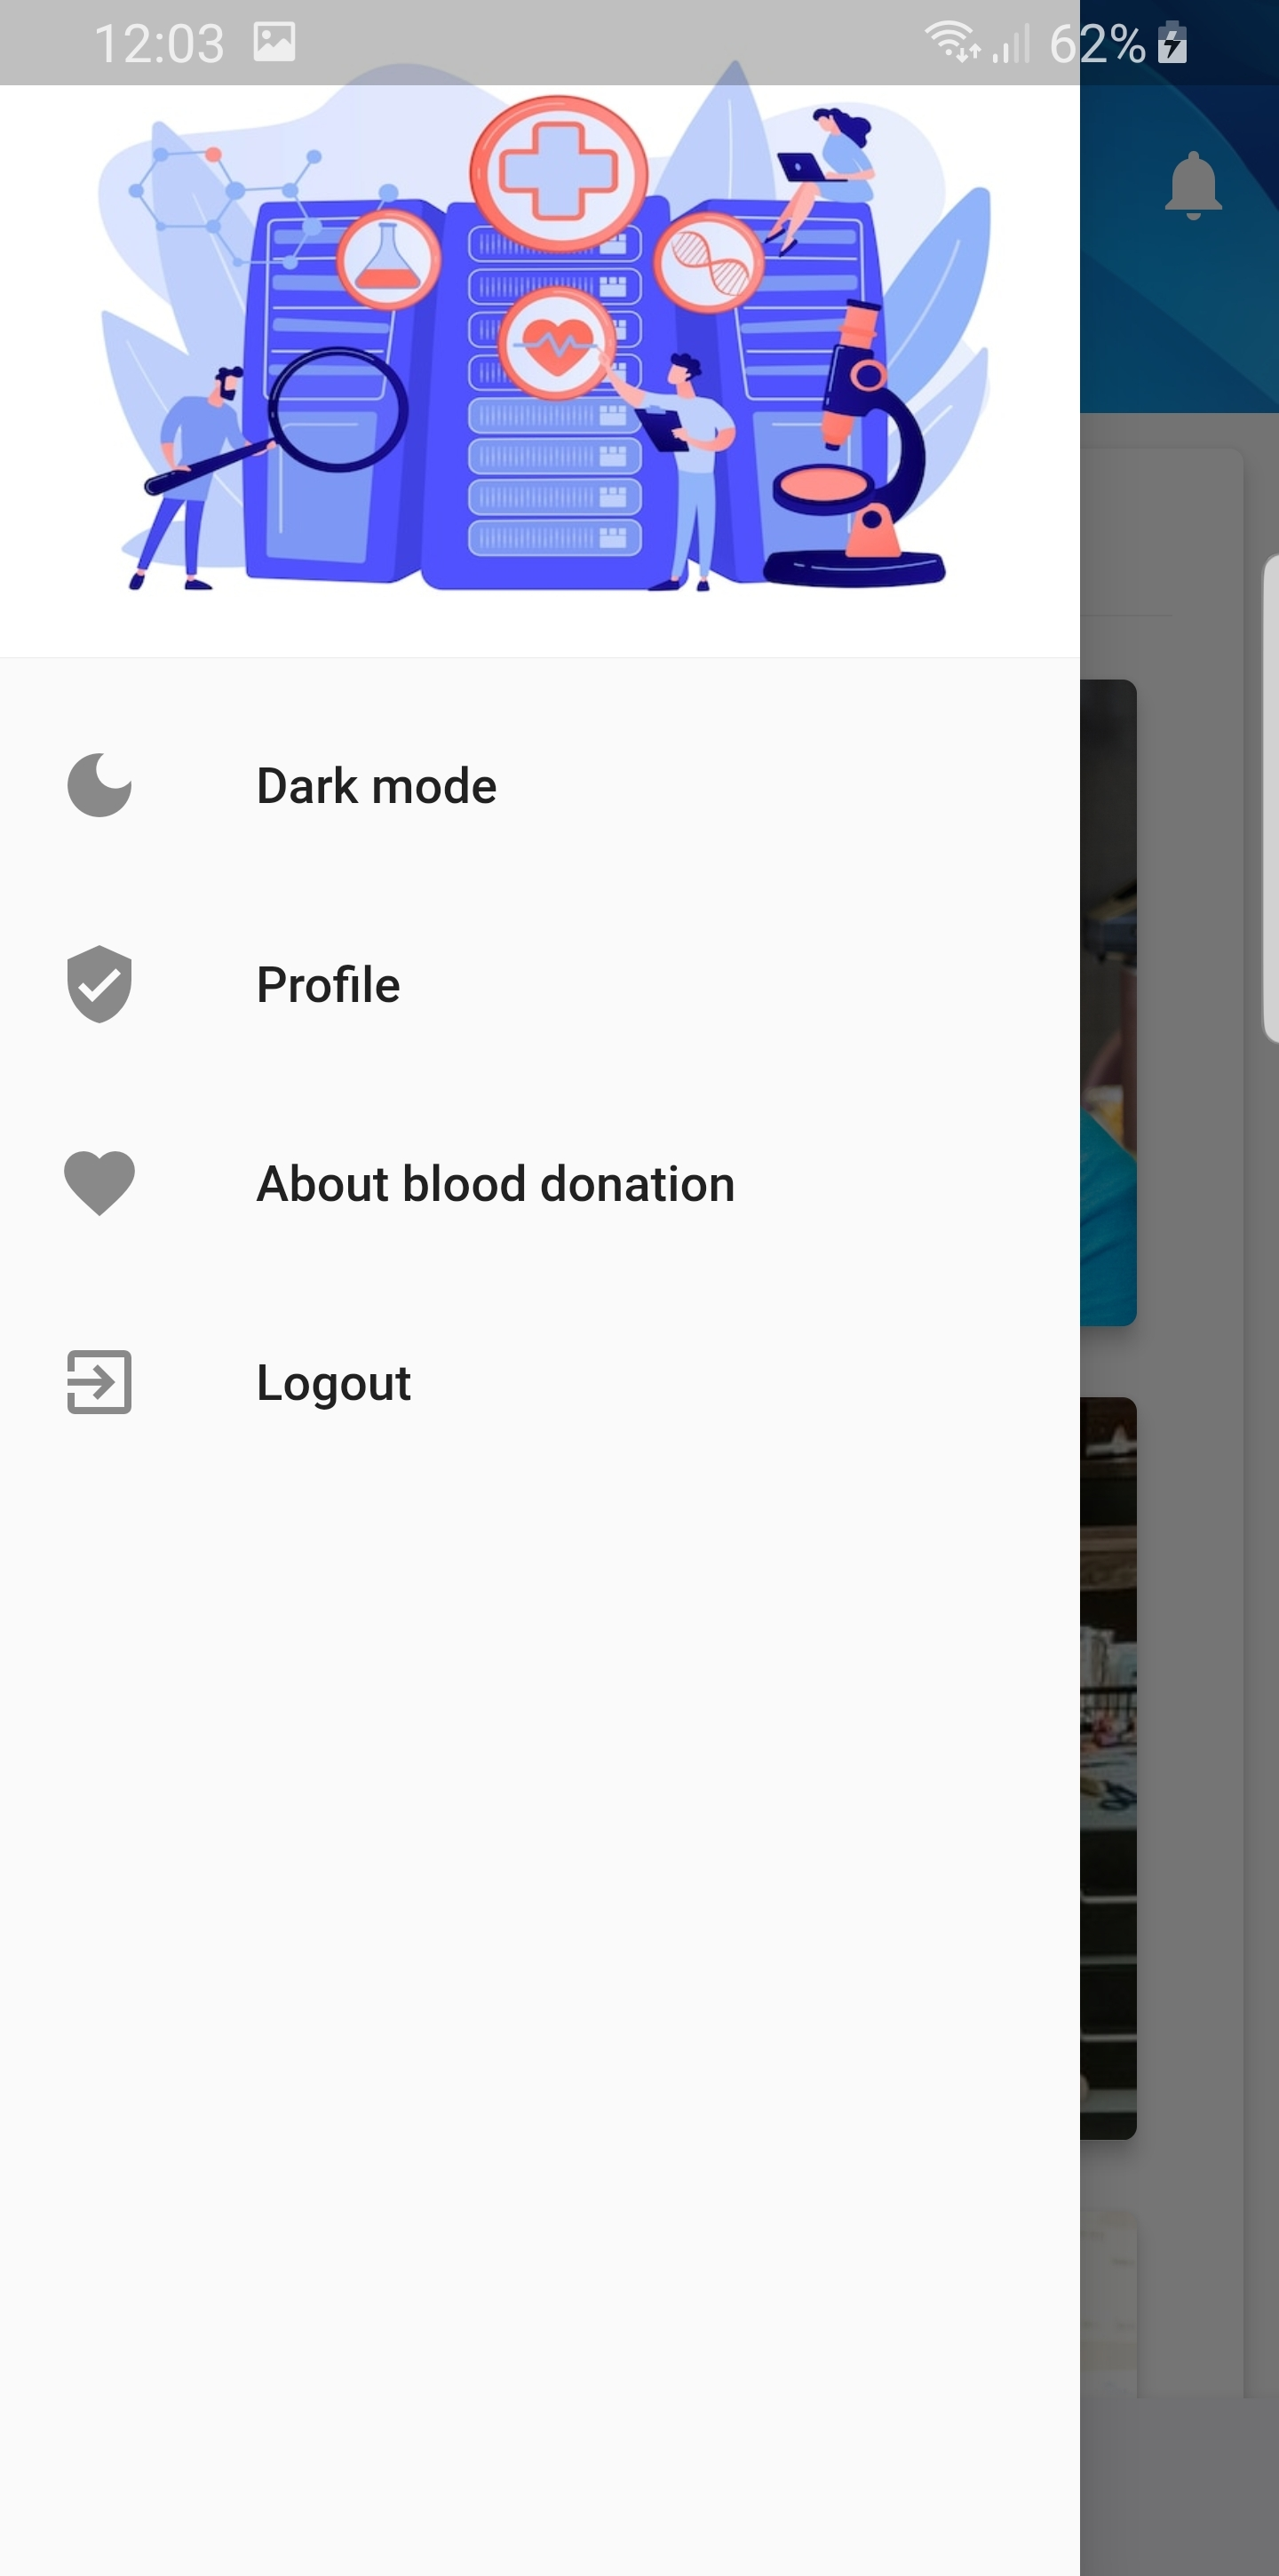
\includegraphics[width=\linewidth]{images1/sidebardonor.jpg}
    \caption{Donor side bar}
    \end{subfigure}
    \begin{subfigure}[b]{0.4\linewidth}
        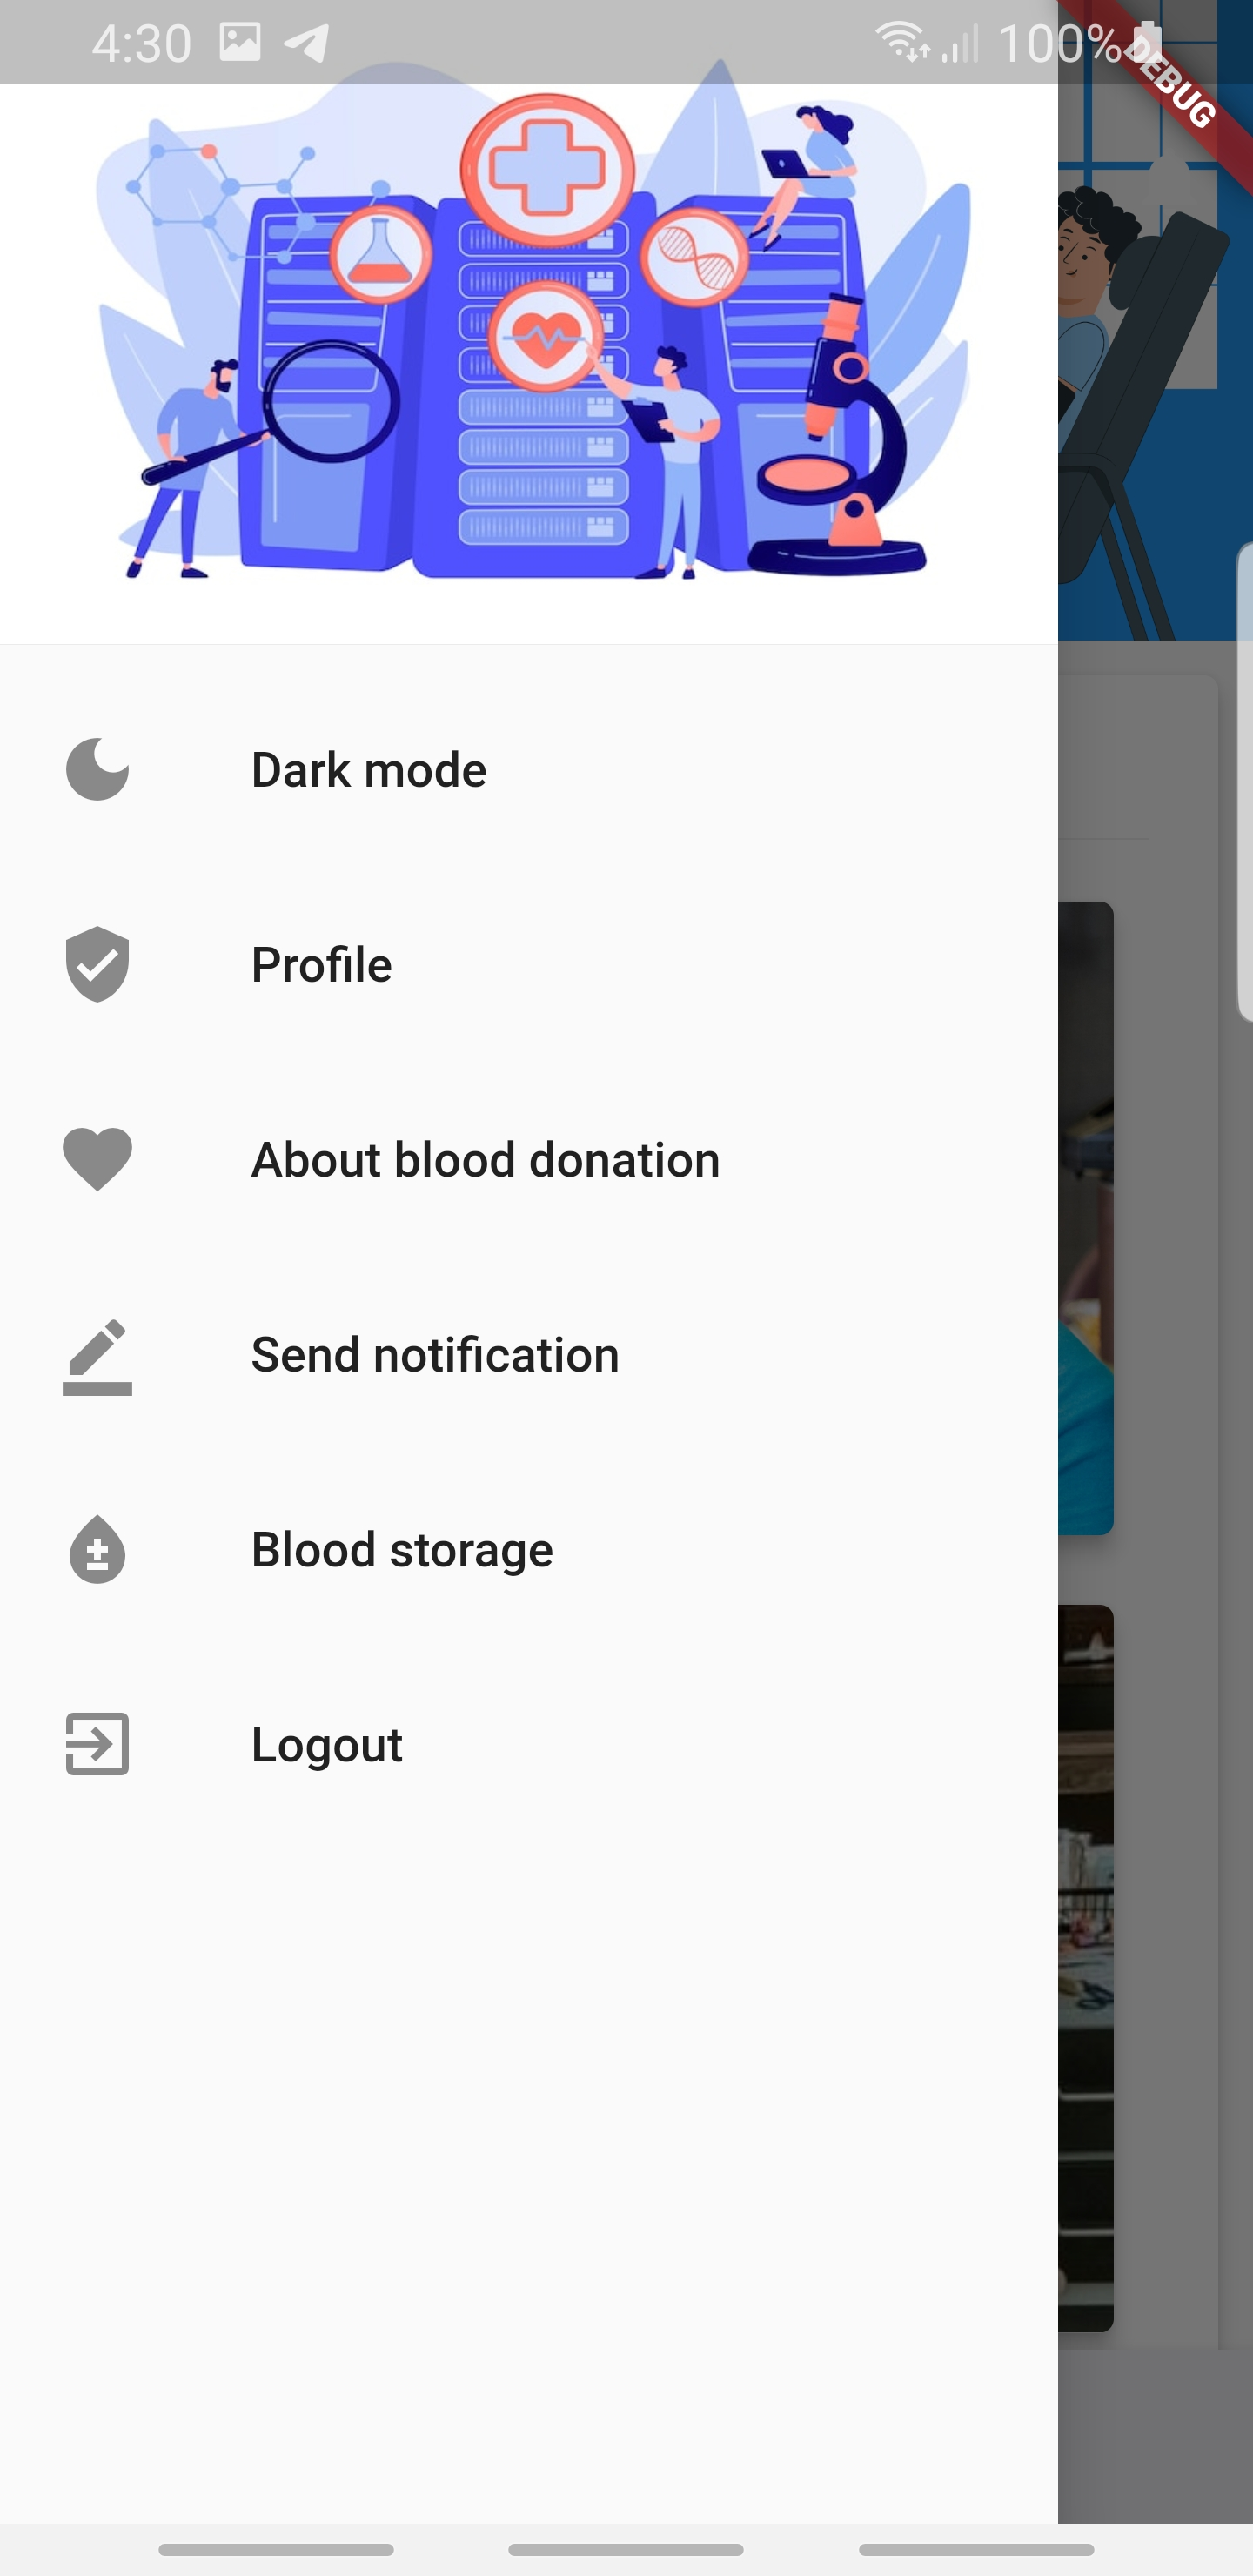
\includegraphics[width=\linewidth]{images1/sidebaradmin.jpg}
    \caption{Admin side bar}
    \end{subfigure}
\caption{Side bars}
\label{fig:distribution}
\end{figure}




\begin{figure}[H]
	\hspace{1cm}
	\begin {minipage}[t]{4cm}
	\centering
	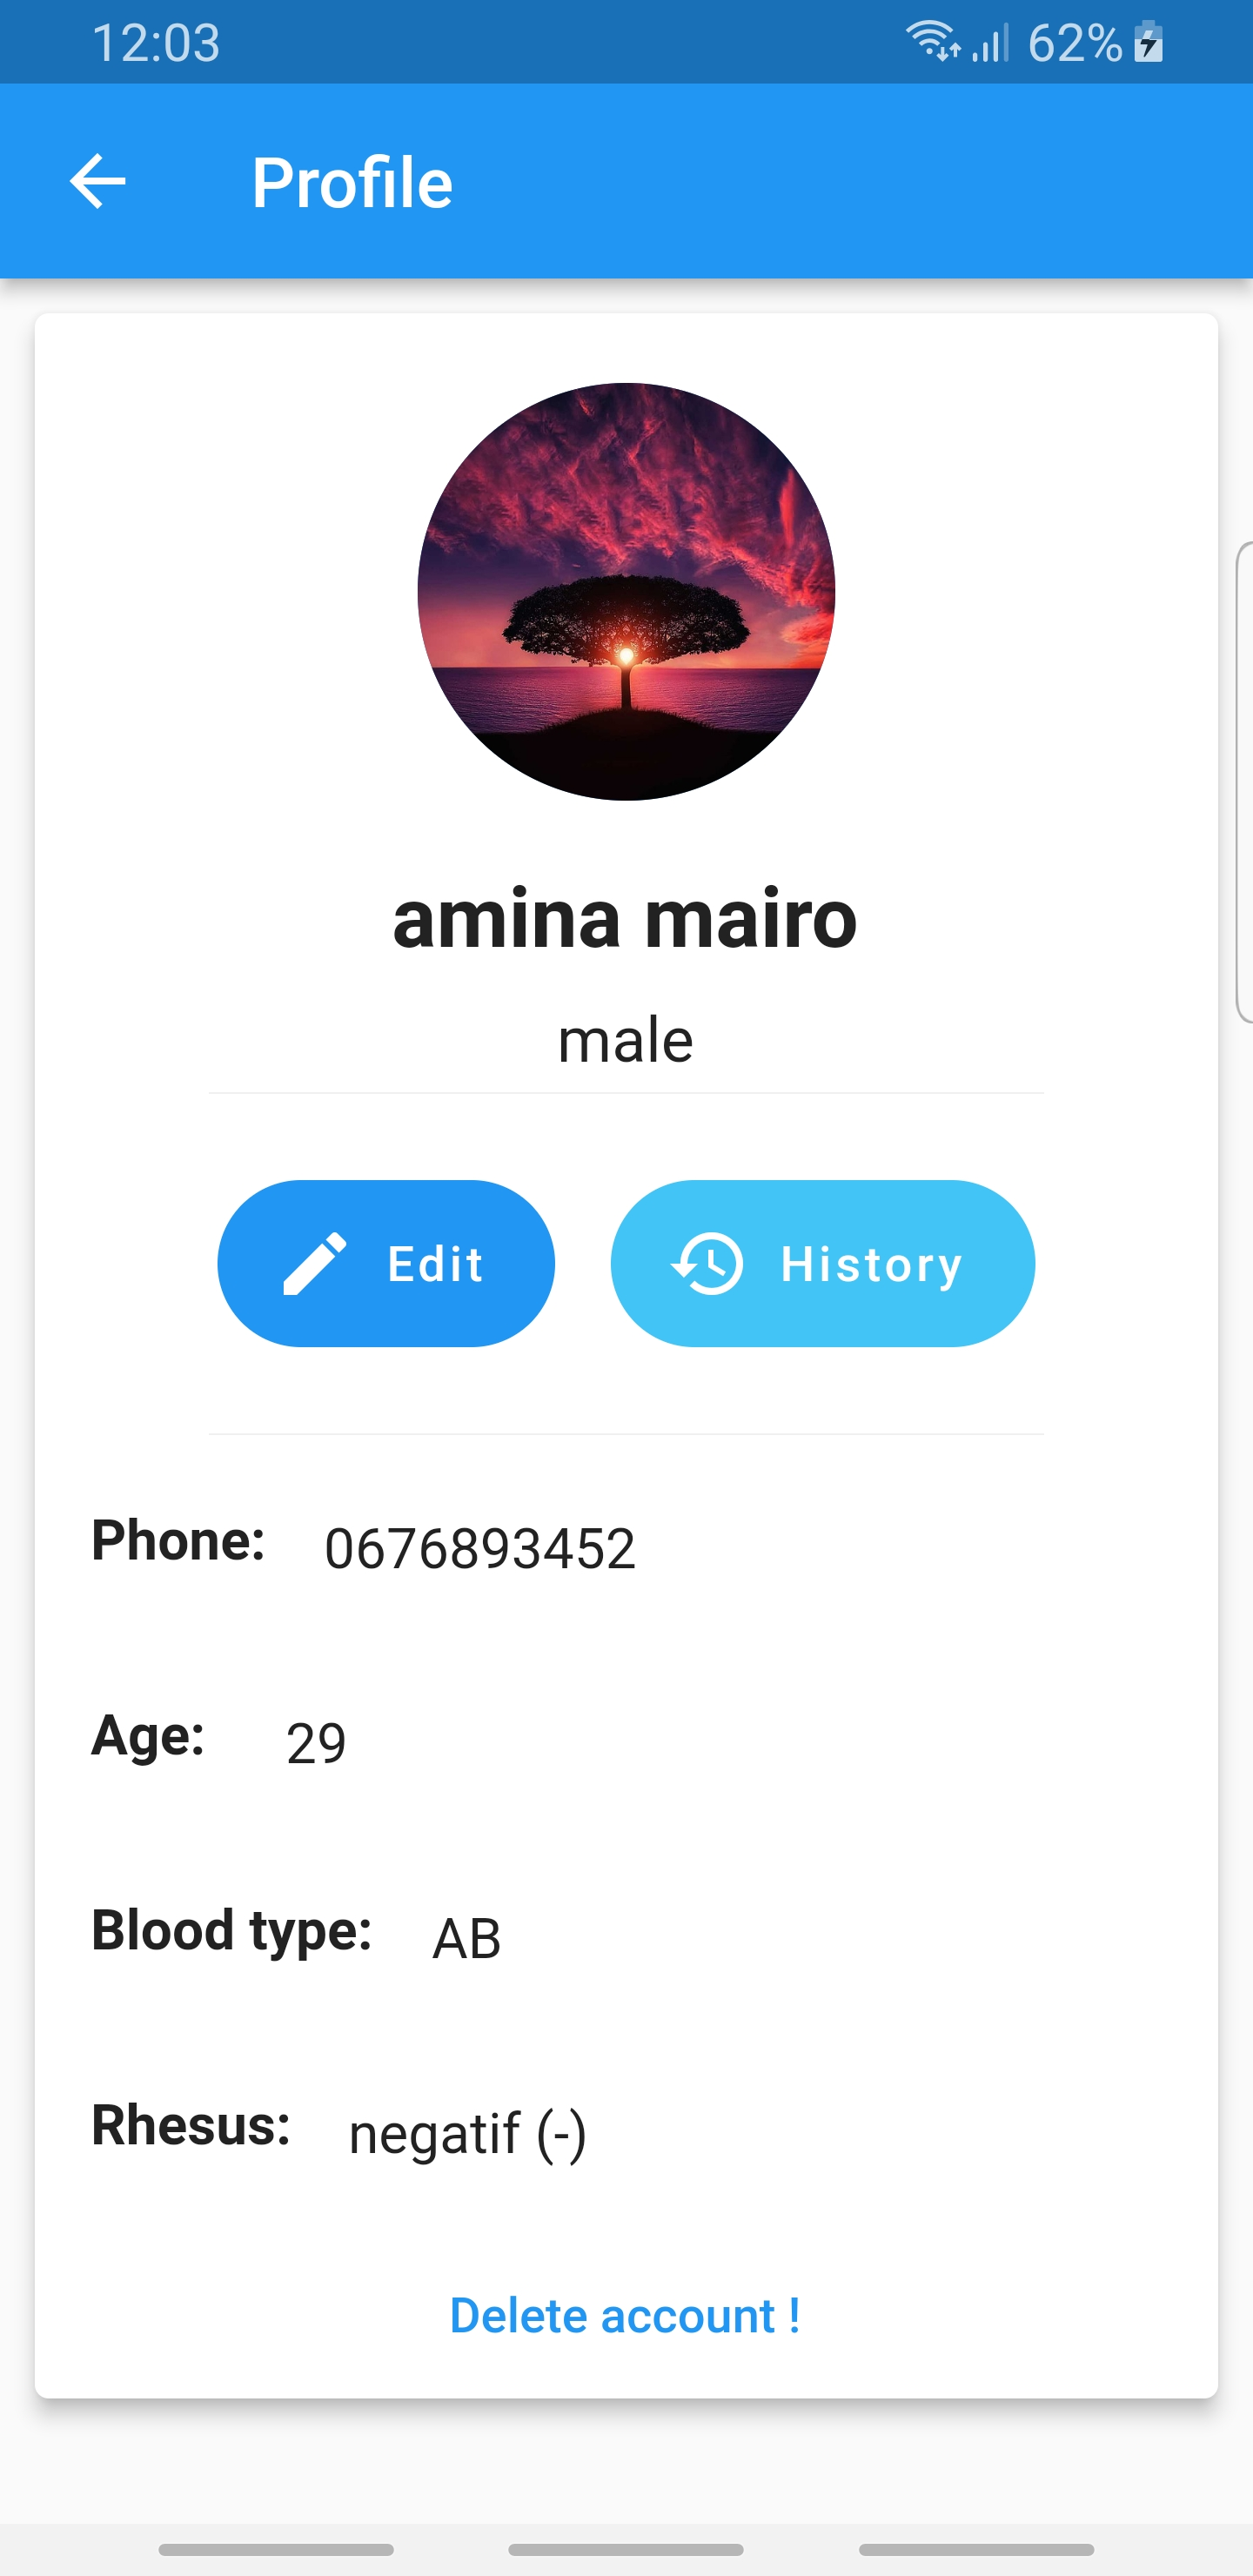
\includegraphics [ width =6 cm ]{images1/profile.jpg}
    \end {minipage}
	\hspace{2.5cm}
	\begin {minipage}[t]{4cm}
	\raggedright
	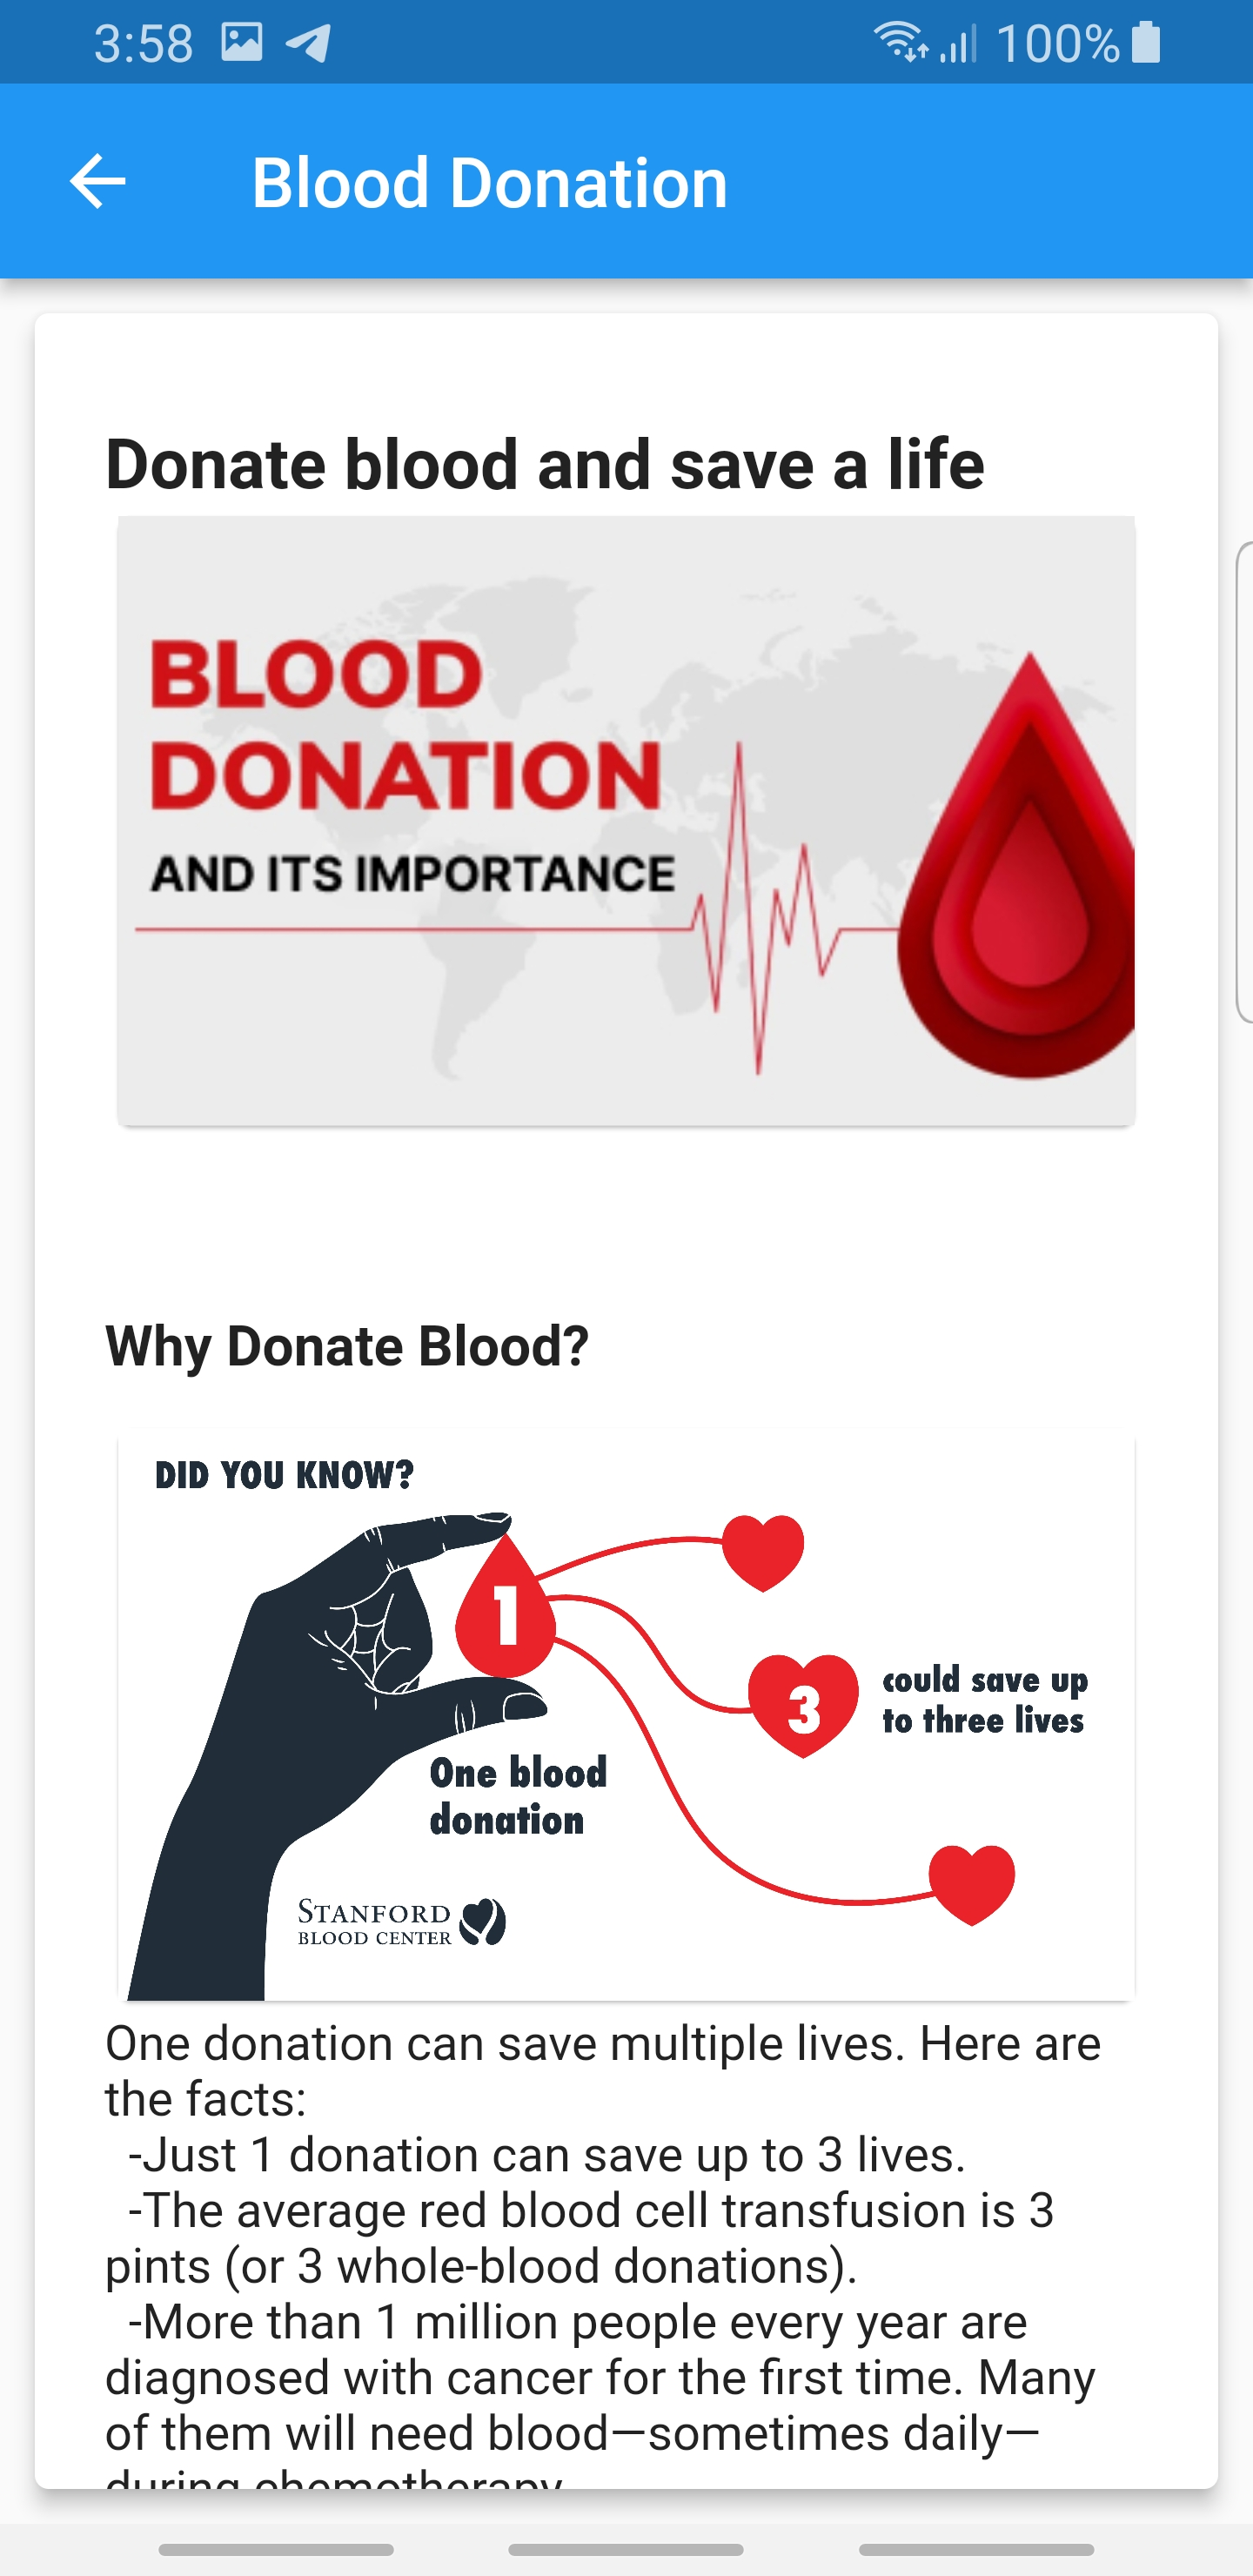
\includegraphics [ width =6 cm ]{images1/aboutbloodd.jpg}
	\end {minipage}
	\caption{Profile and Blood donation}
\end{figure}









\begin{figure}[H]
\begin{subfigure}{.31\textwidth}
  \centering
  % include third image
  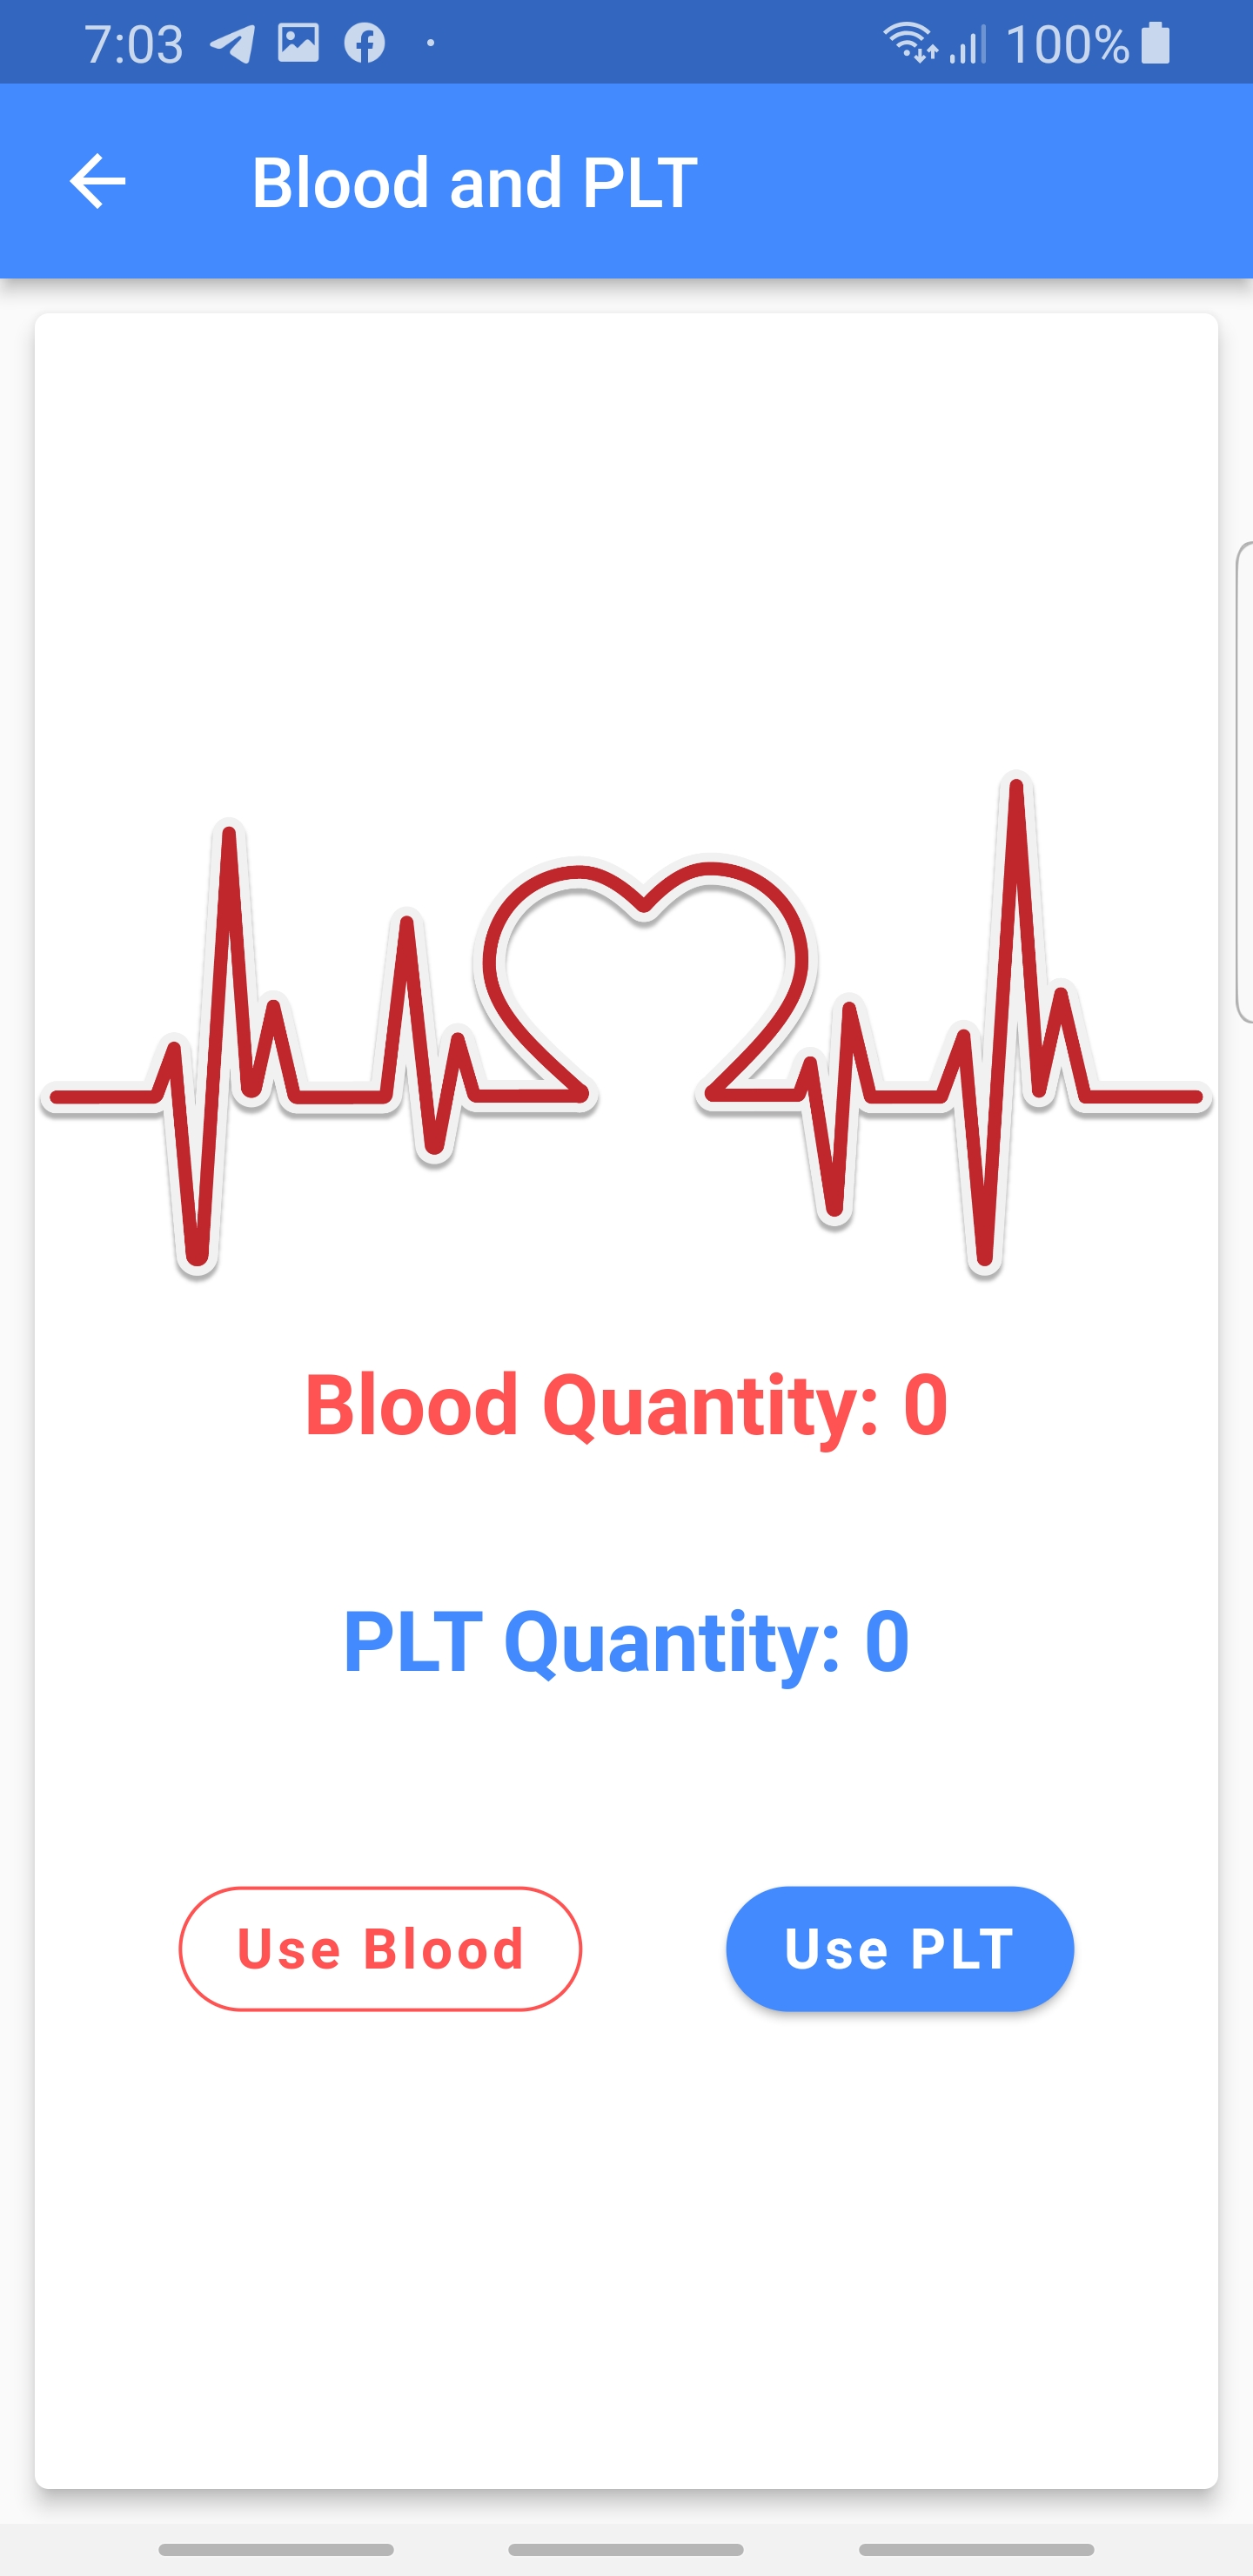
\includegraphics[width=1\linewidth]{images1/stocke.jpg} 
  %\caption{Put your sub-caption here}
  \label{fig:sub-third}
\end{subfigure}
\begin{subfigure}{.31\textwidth}
  \centering
  % include first image
  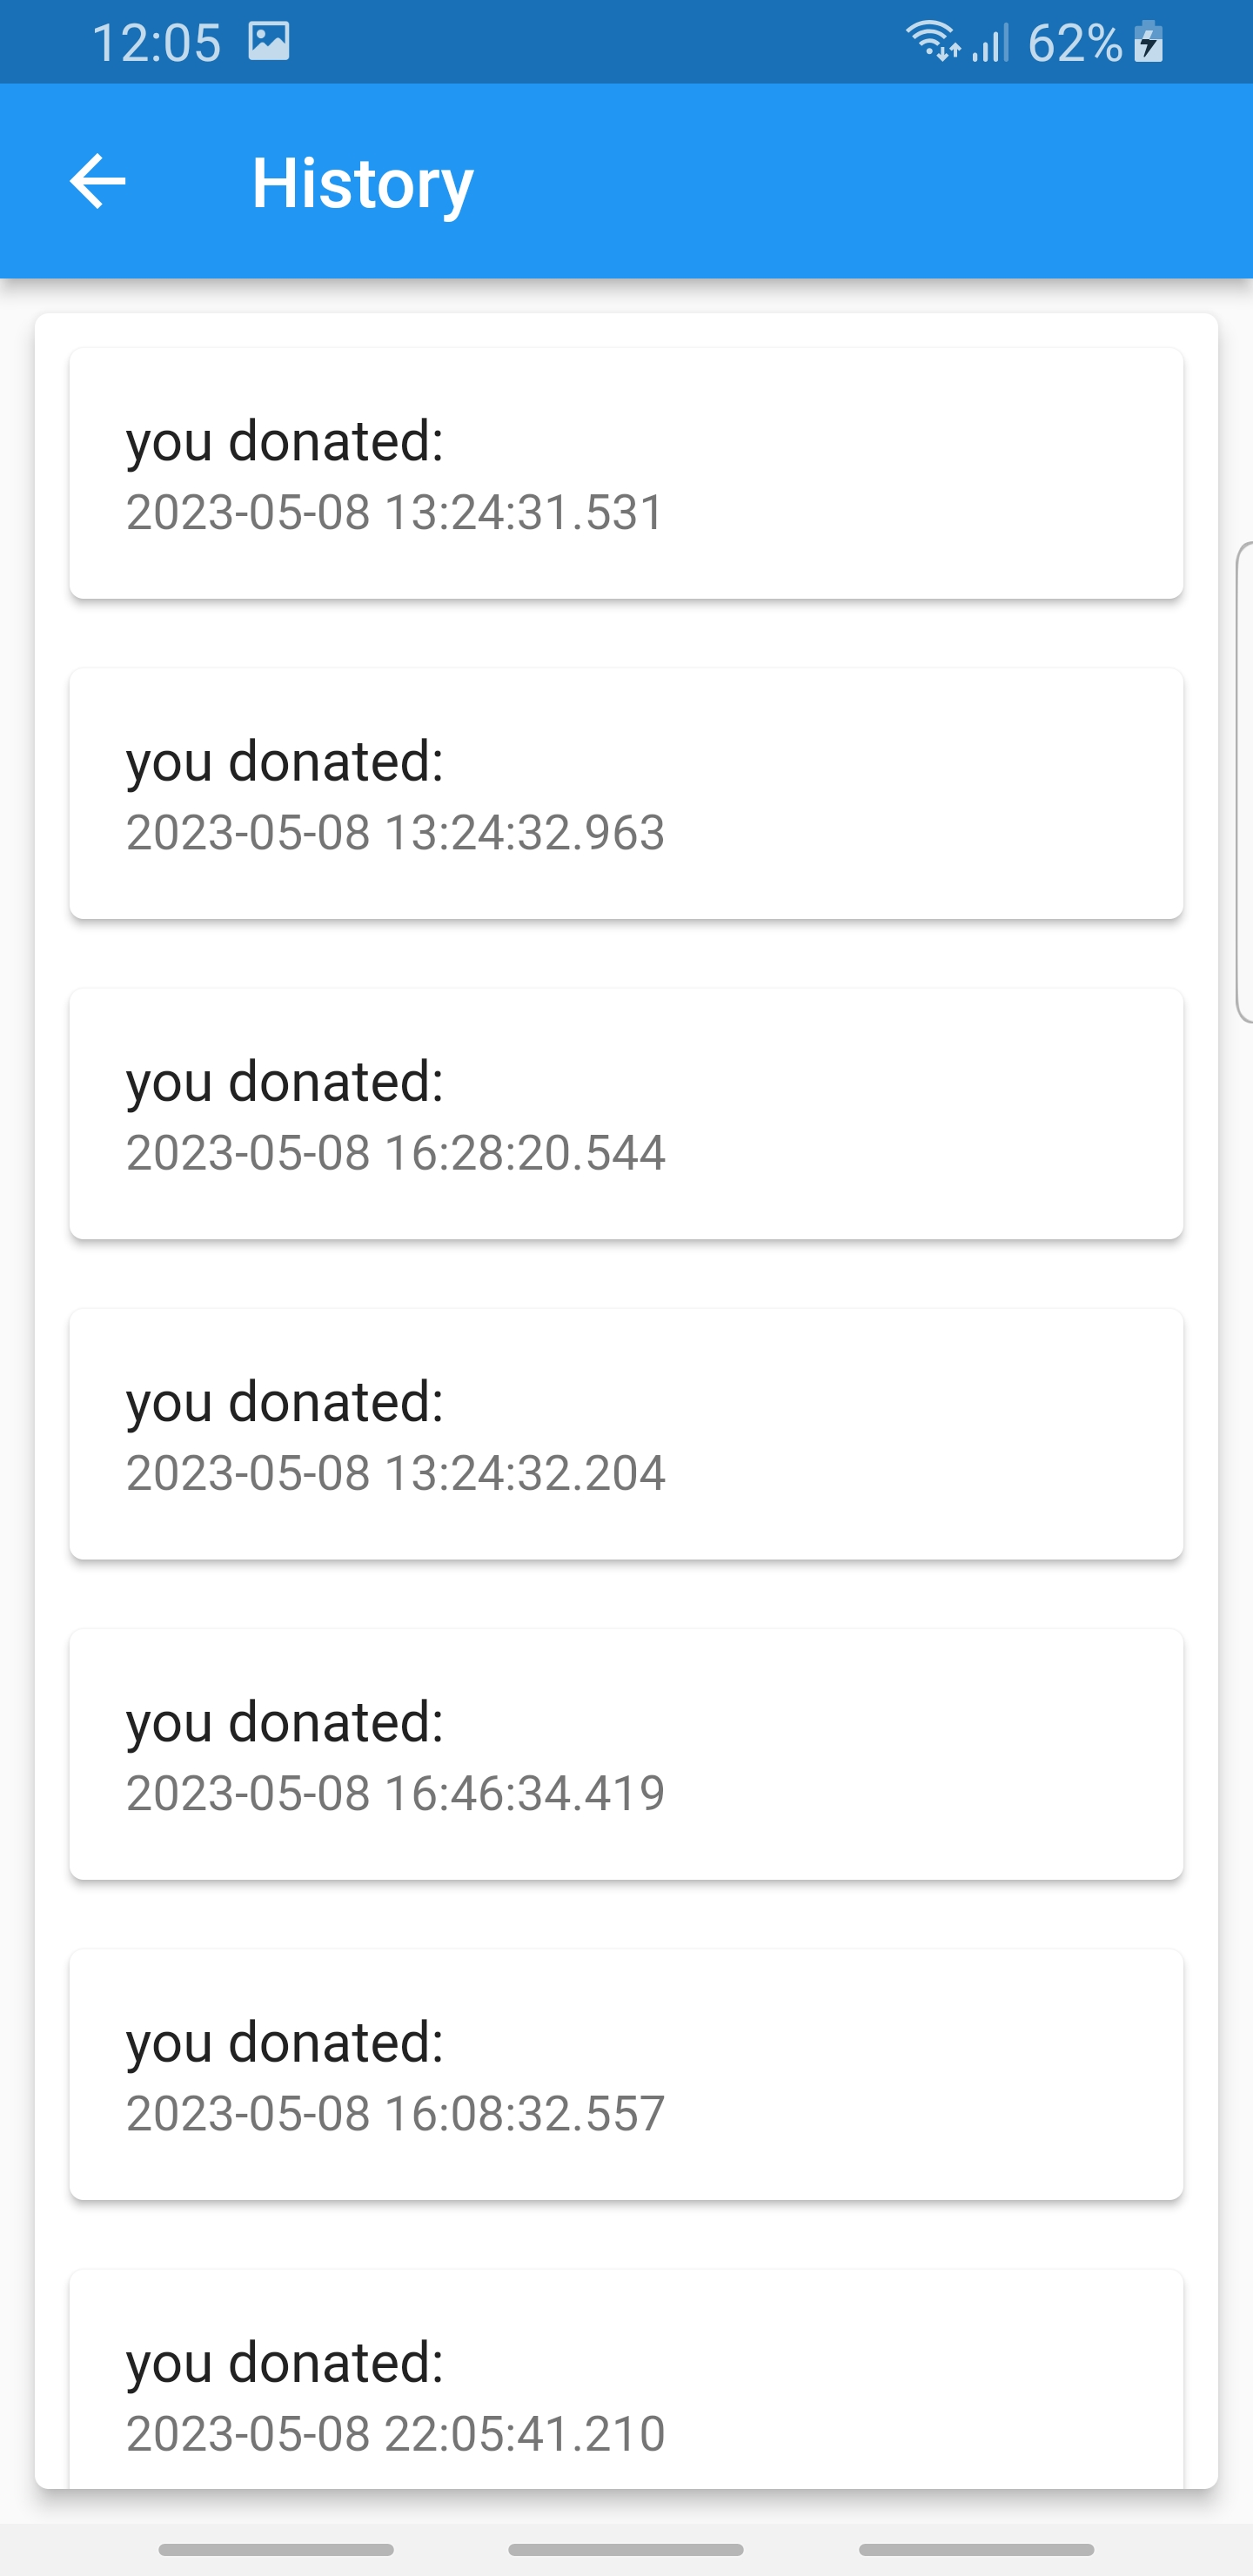
\includegraphics[width=1\linewidth]{images1/history.jpg} 
  %\caption{Put your sub-caption here}
  \label{fig:sub-first}
\end{subfigure}
\begin{subfigure}{.31\textwidth}
  \centering
  % include second image
  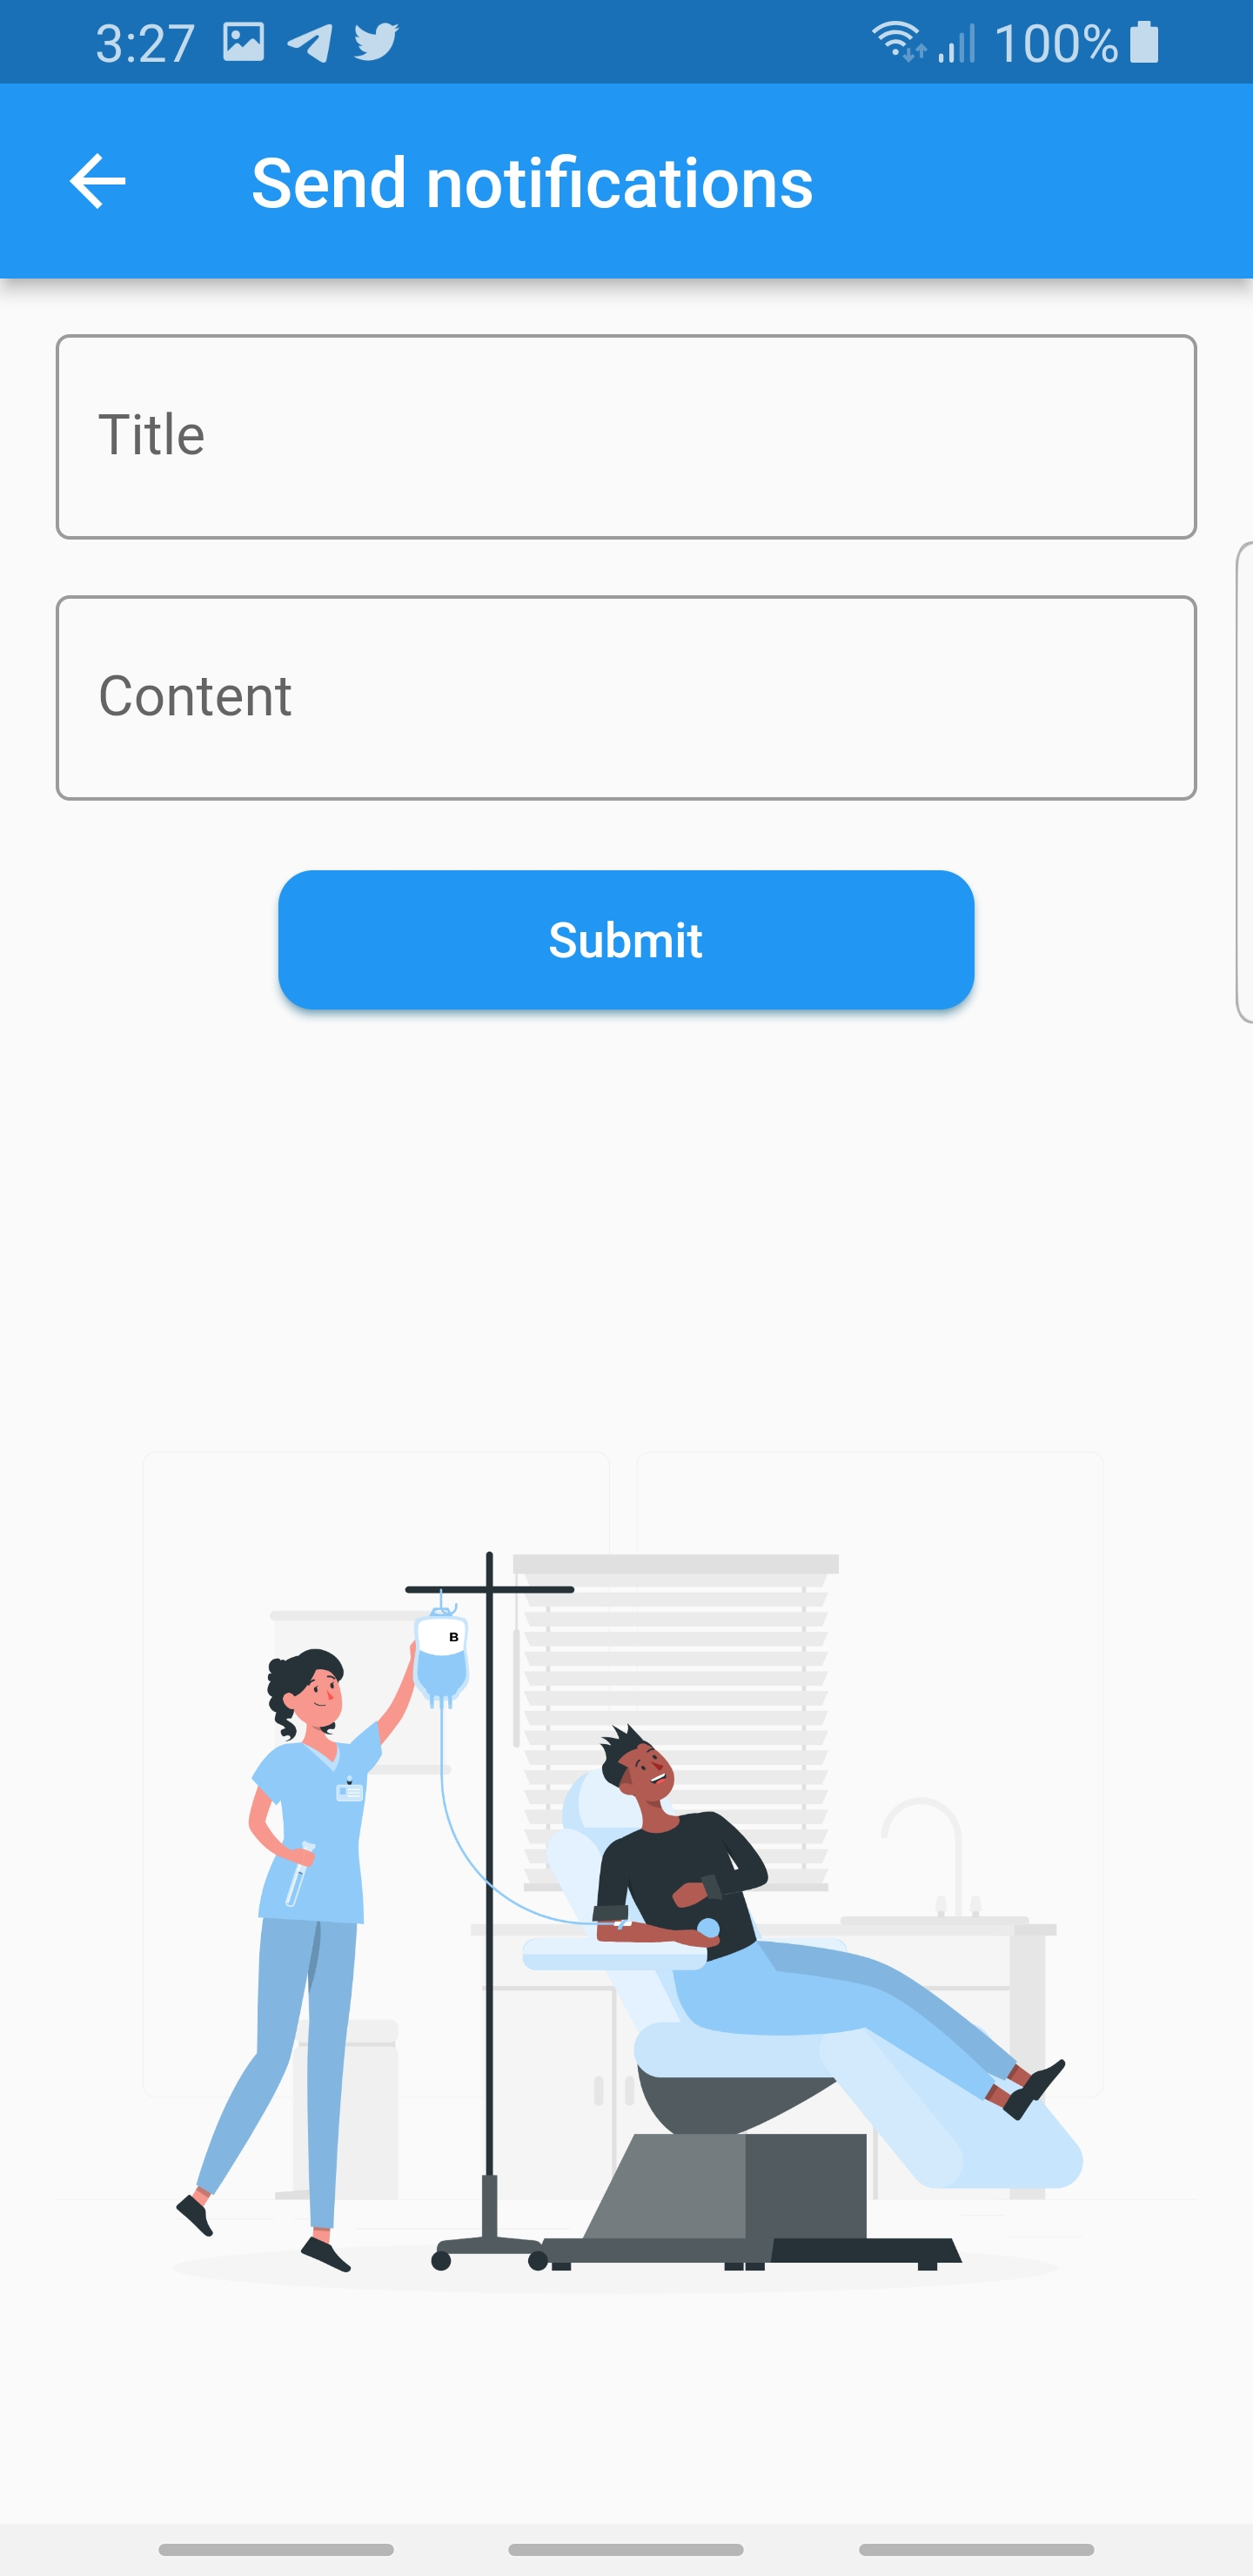
\includegraphics[width=1\linewidth]{images1/sendnotification.jpg}  
  %\caption{Put your sub-caption here}
  \label{fig:sub-second}
\end{subfigure}
%\newline


\caption{More functionalities}
\label{fig:fig}
\end{figure}





\section{Conclusion}
This chapter focused on the implementation process. First, we discussed the tools we used to develop the application, then we talked about the graphic chart and design, and finally, we showed some of the application interfaces with screenshots.

